%%%%%%%%%%%%%%%%%%%%%%%%%%%%%%%%%%%%%%%%%%%%%%%%%%
%% Bachelor's & Master's Thesis Template        %%
%% Copyleft by Dawid Weiss & Marta Szachniuk    %%
%% Faculty of Computing and Telecommunication   %%
%% Poznan University of Technology, 2020        %%
%%%%%%%%%%%%%%%%%%%%%%%%%%%%%%%%%%%%%%%%%%%%%%%%%%


% Szkielet dla pracy licencjackiej pisanej w języku polskim.

\documentclass[english,masters,a4paper,oneside]{ppfcmthesis}


\usepackage[utf8]{inputenc}
\usepackage[OT4]{fontenc}

% Fix footnotes to the bottom of the page
\usepackage[bottom, perpage]{footmisc}

% Better table formatting
\usepackage{makecell}               % Makecell for breaking a long text
\renewcommand{\cellalign}{tl}       % Makecell left alignment
\renewcommand{\arraystretch}{1.75}  % More vertical padding

% Code snippets
\usepackage{listings}
\usepackage{color}

\usepackage{multicol}

\usepackage{caption}
\usepackage{subcaption}
\usepackage{multirow}

\usepackage{pdfpages}

\definecolor{codegreen}{rgb}{0.00,0.60,0.00}
\definecolor{preprocesorbrown}{rgb}{0.50,0.25,0.23} 
\definecolor{codelightblue}{rgb}{0.30,0.70,0.60}

\lstset{frame=tb,
  aboveskip=3mm,
  belowskip=3mm,
  showstringspaces=false,
  columns=flexible,
  basicstyle={\small\ttfamily},
  numbers=none,
  numberstyle=\tiny\color{gray},
  keywordstyle=\color{codelightblue},
  commentstyle=\color{codegreen},
  stringstyle=\color{preprocesorbrown},
  breaklines=true,
  breakatwhitespace=true,
  tabsize=2,
  captionpos=b
}

% Lists without bulletpoints
\usepackage{enumitem}

\lstdefinestyle{lstC}
{
	language = C,
	keywordstyle     =   \color{blue}\ttfamily,
  	commentstyle     =   \color{codegreen}\ttfamily,
  	stringstyle      =   \color{red},
  	emphstyle        =   \color{codelightblue}\ttfamily,
  	directivestyle   =   \color{preprocesorbrown}\ttfamily,
     morekeywords   =   {inline, target_ulong, uint32_t, uint64_t, no_inline, BOOL, _Bool},
}

\lstdefinestyle{lstCsharp} 
{
	language = C++, % No C# support
	keywordstyle     =\color{blue}\ttfamily,
  	commentstyle     =\color{codegreen}\ttfamily,
  	stringstyle      =\color{red},
  	emphstyle        =\color{codelightblue}\ttfamily,
  	directivestyle   =\color{preprocesorbrown}\ttfamily,
  	morekeywords     ={var,async,await,using,byte,string,get,set,uint, checked},
  	emph             ={Descendants,First,FormUrlEncodedContent,HttpClient,
  					   HttpWebRequest,HttpWebResponse,JObject,JProperty,
  					   KeyValuePair,Length,List,OfType,
  					   PropertyChangedEventHandler,Stream,StreamReader,
  					   Value,WebRequest,Where}
}

%--------------------------------------
% Strona tytułowa
%--------------------------------------

% Autorzy pracy, jeśli jest ich więcej niż jeden
% wstaw między nimi separator \and
\author
{%
   Patryk Kościk \album{144635}
}
\authortitle{}                                % Do not change.

\title
{%
   Analysis of Trace-Based Evaluation of Cache Usage on the Example of the Renode Framework
}

% Your supervisor comes here.
\ppsupervisor{dr inż. Mariusz Naumowicz} 

% Year of final submission (not graduation!)
\ppyear{2024}                                 


\begin{document}

% Front matter starts here
\frontmatter\pagestyle{empty}%
\maketitle\cleardoublepage%

%--------------------------------------
% Miejsce na kartę pracy dyplomowej
%--------------------------------------

\thispagestyle{empty}\vspace*{\fill}%
\begin{center}Tutaj będzie karta pracy dyplomowej;\\oryginał wstawiamy do wersji dla archiwum PP, w pozostałych kopiach wstawiamy ksero.\end{center}%
\vfill\cleardoublepage%


% \thispagestyle{empty}\vspace*{\fill}%

\begin{vplace}

\begin{center}
   \huge{\textit{Abstract}}
\end{center}

% TODO: proofread
In the context of modern computing, CPU cache plays a pivotal role in defining
system performance across both complex computing systems and edge/embedded solutions.
%
Consequently, considerable effort is being invested in enhancing cache
implementations and various optimizations, aimed at supporting both
extensive workloads, such as large machine learning models, and smaller, more
time-sensitive workloads, such as improving latencies in real-time operating
systems.
%
This work will focus on determining whether using trace-based approaches are an
effective solution for profiling CPU cache usage and performance.
%
Additionally, this study will examine the effects of cache size and configuration
on processing bottlenecks, offering insights into how these factors influence
overall system performance.

\end{vplace}

\newpage

\begin{vplace}

\begin{center}
   \huge{\textit{Streszczenie}}
\end{center}

% TODO: proofread
W kontekście nowoczesnych systemów komputerowych, pamięć podręczna procesora
odgrywa kluczową rolę w wydajności systemu, zarówno w złożonych
systemach obliczeniowych, jak i rozwiązaniach brzegowych/wbudowanych.
%
W związku z tym pokładane jest dużo pracy w ulepszanie implementacji pamięci
podręcznej i różne optymalizacje, mające na celu wspieranie zarówno złożonych
obliczeniowo zadań, takich jak duże modele uczenia maszynowego, jak i
mniejszych, bardziej wrażliwych na czas obciążeń, takich jak optymalizacja
opóźnień w systemach operacyjnych czasu rzeczywistego.
%
Ta praca skupi się na określeniu, czy wykorzystanie podejścia opartego
na śledzeniu jest skutecznym rozwiązaniem do profilowania wykorzystania i
wydajności pamięci podręcznej procesora.
%
Dodatkowo, to badanie zbada wpływ rozmiaru i konfiguracji pamięci podręcznej na
wąskie gardła przetwarzania, oferując wgląd w to, jak czynniki te wpływają na
ogólną wydajność systemu.

\end{vplace}

\newpage

%--------------------------------------
% Spis treści
%--------------------------------------

\pagenumbering{Roman}\pagestyle{ppfcmthesis}%
\tableofcontents* 
\cleardoublepage % Zaczynamy od nieparzystej strony

%--------------------------------------
% Rozdziały
%--------------------------------------

%Najwygodniej jeśli każdy rozdział znajduje się w oddzielnym pliku
\mainmatter%

\chapter{Introduction}

\section{Motivation and goals of the thesis}
%

\section{Thesis organization}
%


\chapter{Background}


\section{System emulation}
%

\section{Caches and memory hierarchies}
\subsection{Overview of memory hierarchy}
\subsection{Role of caches in system performance}
%

\section{CPU caches}
\subsection{Basic configuration parameters}
%
\subsection{Placement policies}
Cache placement policies determine where a specific memory block can be loaded into
the cache. The choice of placement policy influences the cache architecture and
its control logic - affecting the overall complexity and performance of the system.
Each policy involves trade-offs between speed, by the means of reducing cache misses and
thrashing, and hardware costs related to the size and design of the hardware.

\subsubsection{Fully associative cache}
In the fully associative cache, each \textit{cache line} can hold a copy of
\textit{any memory location}.
% TODO: image, diagram



\subsubsection{Set associative cache}
The set associative cache introduces a concept of a \textit{set} - a collection
of more than one cache line.
% TODO: image, diagram

\subsubsection{Directly mapped cache}
In the directly mapped cache, each \textit{cache line} can hold a copy of
a single \textit{tag}.
% TODO: image, diagram

%
\subsection{Replacement policies}
\subsubsection{Queue based}
\subsubsection{Recency based}
\subsubsection{Frequency based}
%
\subsection{Cache coherency}
\subsubsection{Direct memory access}
\subsubsection{Symmetric multiprocessing}
%


\chapter{State of the art} % XXX: EXTREMELY_NASTY: i might've misunderstood the point of this section, should _academic_ papers be reviewed here? anyways,
% this section will need some elbow grease to "fit in" into the definition of the "state of the art"
% PZIE: I think it can be about "what is out there"

\section{Whole system emulators}
% PZIE Full system simulation is a coined phrase

\subsection{Renode}

The Renode framework is Antmicro’s open-source, permissively licensed (MIT), embedded device simulation platform. Being mostly written in C\# and C, the framework provides an organized,
% PZIE I'd cite Renode with a link
easily expandable codebase, rich in object-oriented principles. It can be compiled using both mono and .NET build systems for all major operating systems.
The framework supports a wide range of CPU architectures, including, among others, \textit{ARMv7}, \textit{ARMv8}, and \textit{RISC-V}.
Additionally, Renode offers comprehensive whole-system emulation, allowing for the simulation of complex peripherals and interconnections. This capability enables developers to
create and test realistic embedded system environments, including I/O devices, sensors, and communication interfaces. The platform description files and execution scripts
use simple and easily modificable syntax, allowing for rapid iteration, efficient testing, and seamless integration with various development workflows.

Some of the outstanding qualities of the Renode framework are its advanced debugging, logging, and execution tracing systems, such as:
\begin{itemize}
	\item \textbf{Execution tracer:} this subsystem allows for monitoring and saving the traces of all major CPU operations, including execution tracing, memory access logging and
		performed I/O operations.
	% PZIE execution traces includes execution tracing?
	\item \textbf{Execution metrics:} a module that allows to measure quantitative data related to the simulation, including number of accesses to peripherals, number of exceptions and
		the number of executed instructions (including counting of specific opcodes).
	\item \textbf{Execution profiler:} a call stack analysis tool intended for debugging and inspecting the guest virtual machine software.
	\item \textbf{Python hooks:} the framework utilizes a built-in Python API to provide an easy entry point to automate testing, extend the simulator's functionalities, and integrate
		seamlessly with other tools and workflows.
\end{itemize}

\noindent Due to its advanced debugging capabilities, the Renode framework was selected as the emulation framework for this work.

\subsection{QEMU}

QEMU, also called \textit{Quick Emulator} \cite{qemuoriginal}, is a whole-system emulation framework with KVM support. Originally developed by Fabrice Bellard \cite{qemufabrice} and released
under GNU General Public License v2. It is written entirely in the C programming language, and can compiled for all major operating systems.

It supports most popular CPU architectures and is capable of whole system emulation.
% PZIE: you said about the whole system already
However, unlike in Renode, platforms in QEMU are defined in \textit{header files}, which means
that changes to the platform configuration are relatively slow and require recompilation of the project. Another similarity to Renode is that QEMU also provides a set of debugging
and analysis tools. However, instead of using Python as a scripting engine, QEMU implements its own fully custom plugin system, which also requires the user to recompile the
application to apply changes. Its main distinguishing factor is built-in support for userspace and KVM emulation, allowing for very efficient emulation if the simulated software is
compiled for the same architecture and/or operating system. In the context of this thesis, QEMU ships with a \textit{Cache Modelling TCG Plugin} \cite{tcgcachemodelling}.

% XXX: i don't like this, this is supposed to be an overview of the state of the art... and I'm showing off 2 simulators that are somewhat "popular",
% and putting the rest into a "catch-all bin". In the ideal world I'd not do that, but to be frank, I don't really know what I should describe here, as I'm not
% that familiar with them...
% PZIE: My suggestion - ask mnaumowicz. I think it's ok tbh
\subsection{Other notable simulators}

\begin{itemize} % TODO: add more info here
	\item \textbf{Intel Simics:} is a full-system simulator developed by Wind River, a subsidiary of Intel. Simics supports a wide range of CPU architectures and peripheral models.
		It is released under a proprietary, closed-source license.
	\item \textbf{gem5:} event driven full-system emulator, mainly used in academia and advanced research institutions. Developed by universities, companies and the community, maintained by the
		\textit{Project management committee} \cite{gem5governance}. % TODO: gem5 is mainly used in the academia, it is pretty advanced, but hard to use for a "newcomer", I have no idea how to put this nicely
		% PZIE: lgtm, but then you have it just below again in more detail
\end{itemize}

\section{Cache simulators}

\subsection{gem5}

The \textit{gem5} project is a highly flexible, modular platform for computer system architecture research and development that includes advanced cache modeling features \cite{gem5cachesupport}.
It has been previously used in a number of academic papers discussing the topic of CPU caches \cite{gem5cachecite1, gem5cachecite2, gem5cachecite3}.

This simulator supports a wide range of cache architectures and configurations, offering high flexibility, essential for research and academic institutions \cite{gem5}.
It operates with cycle-level simulation accuracy, allowing for modeling and measuring the timing performance characteristics of cache behavior. This potentially provides a higher level of accuracy
compared to behavioral or functional simulators \cite{gem5accuracy}. \textit{gem5} enables simulation of complex memory hierarchies, including multi-level caches, which are commonly
used in modern computer architectures \cite{gem5multilevel, cachesimsurv}.

Despite its strengths, the high level of detail and flexibility in 
% PZIE: in what?
can make it complex and difficult to set up. The documentation is extensive, but its high level of detail can be overwhelming,
making it challenging to navigate effectively \cite{gem5hell}. The complex simulation model also requires significant computational resources for support advanced, real world payloads
\cite{gem5, cachesimsurv}. As an open-source and mainly community and academia backed project, \textit{gem5} relies on community updates and maintenance, which can lead to periods where certain
features may be underdeveloped or not fully supported \cite{gem5hell, gem5maintainers}.
% PZIE: Frankly speaking, this last sentence is triggering. You mention open source like it's a bad thing. Does not really give us anything
While the project uses a modular approach for its modules and hardware models, the project complex codebase,
unstable APIs, frequent functionality breaking changes \cite{gem5hell} result in the fact that \textit{gem5} is very hard to integrate with external tooling.
% PZIE having said that, I have no probem with this part

\subsection{QEMU TCG Cache Modeling plugin} \label{sec:qemu_cache}

The TCG Cache Modeling plugin is a plugin for the QEMU emulator, created as a part of Google Summer of Code \cite{qemucachegsoc}. It supports a variety of cache configuration parameters, such as
cache and block size, eviction policies and optional L2 support \cite{tcgcachemodelling}.

A significant advantage of the plugin is its ease of use in the existing QEMU workflows, since it doesn't require any additional software to be introduced into the development processes.
However, such integration makes it nearly impossible to integrate this cache analysis tool with other simulators. There is no functionality to save the trace files, and process them off-line,
instead, the entirety of the cache model simulation happens within the constraints of the TCG plugin system \cite{qemutcgplugindocs}, thus begin reliant on QEMU for simulating 
payloads. For users looking for modular cache simulation tools that can be adapted to various other environments, this could pose a significant constraint.

\vspace{10px}
\noindent Efforts have also been made to incorporate cache modeling as a core feature of the QEMU simulator \cite{qemucacheattempt}, but these enhancements have not been merged and the
source code has not been made publicly available.

\subsection{dineroIV}

DineroIV is a cache simulator for memory reference traces, created by the researchers from \textit{University of Wisconsin, Computer Sciences} \cite{dinero}. 
The cache model supports a variety of configuration parameters, such as overall cache size, block size, eviction methods, and others. These parameters are used to define the structure of
single and multi-level caches. DineroIV is purely a cache simulator, with no system emulation backend - it can be only used to emulate the cache from the memory reference traces.
It has been last updated in 1999 and is not available under open source license.

\section{pycachesim}

Pycahesim is a single-core cache hierarchy simulator with Python API and C backend. It has been developed and released by Regionales Rechenzentrum Erlangen, Hochleistungsrechner (RRZE-HPC)
under an AGPL-3.0 license \cite{pycachesim}. The Python API is straightforward and can be easily integrated into external projects. Since the backend is written in a compiled language, it is
relatively fast. The simulator supports complex, multilevel cache configurations, including exclusive and victim caches. % TODO: relative to what? 
However, pycahesim does not support the differentiation of instruction and data caches, which can limit its utility in more complex simulation scenarios. Additionally, the AGPL
license imposes significant restrictions on the commercial use of the project, resulting in little to no industry adoption. Due to this fact, the simulator remains mostly supported
by academic institutions, with very infrequent updates\footnote{As of June 2024, the last update was released over two years ago.}.

\vspace{10px}
\noindent Efforts have been made to integrate QEMU and pycachesim \cite{pycachesimqemu}.

\subsection{Other notable simulators}
% TODO: move items from the list to the sections, explain every one briefly, put some citations, and it shoooould be goooood
\begin{itemize}
	\item \textbf{DynamoRIO, drcachesim:} hard to extract the cache only
	\item \textbf{Cachegrind:} only supports one level of cache
	\item \textbf{libCacheSim:}
	% PZIE: todo above
	\item \textbf{SMPcache:} closed source, windows + gui only
	\item \textbf{CMPsim:} academically published, source code not available
	\item \textbf{CASPER:} academically published, source code not available
\end{itemize}


\chapter{Implementation}

This chapter will cover the details of the cache model, describe its implementation, and provide an overview of the available interfaces and configuration options.
The entirety of the cache model has been implemented in the Python programming language. The motivation for this choice includes the portability of the code, ease of customization and
the ability to rapidly iterate and test different configurations.

\section{Model architecture}

\begin{center}
	\centering
	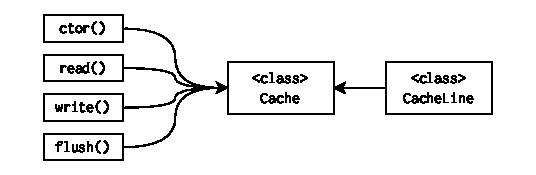
\includegraphics[width=\textwidth]{figures/04-implementation/cache_mdl_arch.pdf}
	\captionof{figure}{Visual representation of the cache model architecture}
	\label{fig:cache_mdl_arch}
\end{center}

\subsubsection{\texttt{Cache}} \label{sec:cache_model}

The Cache class encapsulates the cache memory behavioral model. Besides statistic gathering and helper debug methods, its only public interfaces are methods
providing read/write operations, cache flushing, and a constructor with configuration parameters. The cache configuration is derived from the following inputs:
\begin{itemize}
    \item Cache width: Represents the width of the cache memory, calculated as \(\log_2(\text{cache size})\).
    \item Block width: The width of a cache block, calculated as \(\log_2(\text{block size})\).
    \item Memory width: Denotes the width of the memory address.
    \item Lines per set: The set associativity is defined as $2^n$, where $n \in \{1, 2, 3, ...\}$. A value of -1 indicates fully associative, and a value of 1 indicates direct mapping.
	\item Replacement policy: The line eviction policy that will be used by cache, for example: FIFO, LRU, LFU or Random.
\end{itemize}

\begin{center}
\centering
\begin{minipage}{\linewidth}
\begin{lstlisting}[
    language=Python,
	morekeywords={self},
    label={lst:cache_ctor},
    caption={\texttt{Cache} constructor with configuration parameters}
    ]
class Cache:
    def __init__(
        self,
        name: str,
        cache_width: int,
        block_width: int,
        memory_width: int,
        lines_per_set: int,
        replacement_policy: str | None = None,
        debug: bool = False
    ):
        self.name = name
        self.debug = debug

        # Width of the memories
        self._cache_width = cache_width
        self._block_width = block_width
        self._memory_width = memory_width

        # Convert width to size in bytes
        self._cache_size = 2 ** self._cache_width
        self._block_size = 2 ** self._block_width
        self._memory_size = 2 ** self._memory_width

        self._num_lines = self._cache_size // self._block_size
        self._lines = [CacheLine() for i in range(self._num_lines)]

        if lines_per_set == -1:
            # special configuration case for fully associative mapping
            lines_per_set = self._num_lines

        if not (lines_per_set & (lines_per_set - 1) == 0) or lines_per_set == 0:
            raise Exception('Lines per set must be a power of two (1, 2, 4, 8, ...)')

        self._lines_per_set = lines_per_set
        self._sets = self._num_lines // lines_per_set
        self._set_width = int(math.log(self._sets, 2))

        self._replacement_policy = replacement_policy if replacement_policy is not None else 'RAND'

        # Statistics
        self.misses = 0
        self.hits = 0
        self.invalidations = 0
        self.flushes = 0
\end{lstlisting}
\end{minipage}
\end{center}

\subsubsection*{Read and write cache operations}
\noindent The \texttt{read} and \texttt{write} methods are the primary interface for the cache and have been implemented as follows:

\begin{center}
\centering
\begin{minipage}{\linewidth}
\begin{lstlisting}[
    language=Python,
	morekeywords={self},
    label={lst:cache_write_read},
    caption={\texttt{Cache} write and read interfaces}
    ]
def read(self, addr: int) -> None:
    sset = self._addr_get_set(addr)
    line = self._line_lookup(addr)
    self.printd(f'[read] attempt to fetch {hex(addr)} (set {sset})')

    if line and not line.free:
        self.printd('[read] rhit')
        self.hits += 1
        line.use_count += 1
        line.last_access_time = time.time()
    else:
        self.printd('[read] rmiss')
        self.misses += 1
        self._load(addr)

def write(self, addr: int) -> None:
    sset = self._addr_get_set(addr)
    line = self._line_lookup(addr)
    self.printd(f'[write] attempted write to {hex(addr)} (set {sset})')

    if line:
        self.printd('[write] whit')
        self.hits += 1
        line.last_access_time = time.time()
    else:
        self.printd('[write] wmiss')
        self.misses += 1
        self._load(addr)
\end{lstlisting}
\end{minipage}
\end{center}

\noindent The code responsible for finding matching cache line for the given address has been extracted to the internal\footnote{The Python programming language does not have a
built-in mechanism for enforcing access rights to fields in a class. However, PEP 8 specifies that variables starting with '\texttt{\_}' should be used internally in the class
\cite{pep8}.} \texttt{\_line\_lookup} method:

\begin{center}
\centering
\begin{minipage}{\linewidth}
\begin{lstlisting}[
    language=Python,
	morekeywords={self},
    label={lst:line_lookup},
    caption={\texttt{Cache} line lookup}
    ]
def _get_lines_in_set(self, set_index: int) -> List[CacheLine]:
    line_index = set_index * self._lines_per_set
    return self._lines[
        line_index:
        line_index + self._lines_per_set
    ]

def _line_lookup(self, addr: int) -> CacheLine | None:
    tag = self._addr_get_tag(addr)
    lines_in_set = self._get_lines_in_set(self._addr_get_set(addr))
    return next((line for line in lines_in_set if line.tag == tag), None)
\end{lstlisting}
\end{minipage}
\end{center}

\noindent If a matching line is found, the function returns a reference to this line. If no match can be made, the method returns \texttt{None}. This method uses helper functions
to extract the bit fields from the memory address:


\begin{center}
\centering
\begin{minipage}{\linewidth}
\begin{lstlisting}[
    language=Python,
	morekeywords={self, @staticmethod},
    label={lst:bitfield_hepers},
    caption={Bitfields helper functions}
    ]
@staticmethod
def _extract_bits(value: int, start_bit: int, end_bit: int) -> int:
    num_bits = end_bit - start_bit + 1
    mask = ((1 << num_bits) - 1) << start_bit
    extracted_bits = (value & mask) >> start_bit
    return extracted_bits

def _addr_get_tag(self, addr: int) -> int:
    start = self._block_width + self._set_width
    end = self._memory_width
    return self._extract_bits(addr, start, end)

def _addr_get_set(self, addr: int) -> int:
    start = self._block_width
    end = self._block_width + self._set_width - 1
    return self._extract_bits(addr, start, end)
\end{lstlisting}
\end{minipage}
\end{center}

\subsubsection*{Cache line loading}
\noindent Line loading is facilitated by the \texttt{\_load} method:

\begin{center}
\centering
\begin{minipage}{\linewidth}
\begin{lstlisting}[
    language=Python,
	morekeywords={self},
    label={lst:cache_load},
    caption={\texttt{Cache} load method}
    ]
def _load(self, addr: int) -> None:
    self.printd(f'[load] loading @ {hex(addr)} to cache from Main Memory')
    tag = self._addr_get_tag(addr)
    set_index = self._addr_get_set(addr)
    lines_in_set = self._get_lines_in_set(set_index)

    free_line_index = next((index for index, obj in enumerate(lines_in_set) if obj.free), None)
    if free_line_index is not None:
        index = free_line_index
        self.printd(f'[load] loaded new cache index: {free_line_index} in the set {set_index}')
    else:
        self.printd(f"[load] lines in set {set_index}:")
        self.printd('\n'.join(f'{index}: {line}' for index, line in enumerate(lines_in_set)))
        index = self._select_evicted_index(lines_in_set)
        self.printd(f'[load] invalidated index: {index} in the set {set_index}')
        self.invalidations += 1

    lines_in_set[index].init(tag, False)
\end{lstlisting}
\end{minipage}
\end{center}

\subsubsection*{Line eviction algorithms}
\noindent The line eviction algorithms are implemented in the \texttt{\_select\_evicted\_index} method:

\begin{center}
\centering
\begin{minipage}{\linewidth}
\begin{lstlisting}[
    language=Python,
	morekeywords={self},
    caption={\texttt{Cache} load method}
    ]
def _select_evicted_index(self, lines_in_set: list) -> int:
    if self._replacement_policy == 'RAND':
        return random.randint(0, self._lines_per_set - 1)
    elif self._replacement_policy == 'LFU':
        return min(range(len(lines_in_set)), key=lambda i: lines_in_set[i].use_count)
    elif self._replacement_policy == 'FIFO':
        return min(range(len(lines_in_set)), key=lambda i: lines_in_set[i].insertion_time)
    elif self._replacement_policy == 'LRU':
        return min(range(len(lines_in_set)), key=lambda i: lines_in_set[i].last_access_time)
    else:
        raise Exception(f"Unknown replacement policy: {self._replacement_policy}! Exiting!")
\end{lstlisting}
\end{minipage}
\end{center}


\subsubsection*{Cache flushing}
\noindent Cache flushing is implemented by re-initializing the internal cache state:

\begin{center}
\centering
\begin{minipage}{\linewidth}
\begin{lstlisting}[
    language=Python,
	morekeywords={self},
    label={lst:cache_flush},
    caption={\texttt{Cache} flush method}
    ]
def flush(self) -> None:
    self.printd('[flush] flushing all lines!')
    self.flushes += 1
    self._lines = [CacheLine() for i in range(self._num_lines)]
\end{lstlisting}
\end{minipage}
\end{center}

\subsubsection*{Debugging features}
\noindent The cache class also comes with a set of debugging helpers:
\begin{itemize}
    \item \texttt{print\_addr\_info}: prints address-related information in the specified format (\mbox{binary} or \mbox{hexadecimal}). It displays the address, tag, set, and offset values.
    \item \texttt{print\_cache\_info}: prints details about the cache configuration, including the width of the tag, set, and block fields, as well as the size and number of various cache components.
    \item \texttt{print\_hmr}: prints the hit-miss ratio along with the number of hits, misses, and flushes.
    \item \texttt{print\_debug\_lines}: prints debug information for each cache line, including the tag, whether the line is free, and its use count.
\end{itemize}

\subsubsection{\texttt{CacheLine}}

The \texttt{CacheLine} class represents a cache line entry:

\begin{center}
\centering
\begin{minipage}{\linewidth}
\begin{lstlisting}[
    language=Python,
	morekeywords={self},
    label={lst:cacheline},
    caption={\texttt{CacheLine} class}
    ]
class CacheLine:
    """
    Represents a cache line in a cache set.

    tag (int): The tag of the cache line.
    use_count (int): Used for replacement policies:
    insertion_time (float): The time when the cache line was inserted.
    last_access_time (float): The time when the cache line was last accessed.
    free (bool): Indicates if the line contains valid data.
    """

    def __init__(self):
        self.init()

    def init(self, tag: int = 0b0, free: bool = True):
        self.tag = tag
        self.free = free
        self.use_count: int = 0
        self.insertion_time: float = time.time()
        self.last_access_time: float = 0.0

    def __str__(self) -> str:
        return f"[CacheLine]: tag: {self.tag:b}, free: {self.free}, use: {self.use_count}, insertion: {self.insertion_time}, last access: {self.last_access_time}"
\end{lstlisting}
\end{minipage}
\end{center}

\begin{itemize}
    \item \textbf{Tag:} Binary identifier distinguishing a data block, extracted from its physical address.
    \item \textbf{Use Count:} The line reference usage counter for the LFU replacement policy.
    \item \textbf{Insertion Time:} The timestamp indicating when the cache line was inserted, used by the FIFO replacement policy.
    \item \textbf{Last Access Time:} The timestamp indicating when the cache line was last accessed, used by the LRU replacement policy.
    \item \textbf{Free:} Boolean flag; \texttt{True} if the line is free for new data, \texttt{False} if it contains valid data.
\end{itemize}


\section{Cache interfaces}

The \textit{cache model} (\ref{sec:cache_model}) does not implement any execution, log parsing, and validation logic. This is a deliberate choice to maintain high reusability and modifiability
of the emulation core component. To test and use the cache model, two interfaces were implemented:

\begin{itemize}
	\item \textbf{DummyLogInterface:} a "dummy" interface, intended for usage in test cases. Does not implement any log parsing, instead, the memory accesses are passed as a list of
        memory operations. Does not provide any user-configurable cache parameters options.
    \item \textbf{RenodeLogInterface:} Interface intended to be used with Renode's \textit{ExecutionTracer} log format. Implements a command line interface, allowing for easy cache
        configuration changes, as well as a set of preconfigured cache configurations for a selection of devices.
\end{itemize}


\subsection{\texttt{DummyLogInterface}}

\begin{center}
\centering
\begin{minipage}{\linewidth}
\begin{lstlisting}[
    language=Python,
	morekeywords={self},
    label={lst:dummyinterface},
    caption={\texttt{DummyLogInterface} implementation}
    ]
class DummyLogInterface:
    def __init__(self, cache: Cache):
        self.count_insn_read = 0
        self.count_mem_read = 0
        self.count_mem_write = 0
        self.count_io_read = 0
        self.count_io_write = 0
        self.cache = cache

    def simulate(self, data: list[Dict[str, int]]):
        for access in data:
            for type, addr in access.items():
                match type:
                    case 'mw': # Main memory write
                        self.count_mem_write += 1
                        self.cache.write(addr)
                    case 'mr': # Main memory read
                        self.count_mem_read += 1
                        self.cache.read(addr)
                    case 'ior': # I/O read
                        self.count_io_read += 1
                    case 'iow': # I/O write (flushes cache)
                        self.cache.flush()
                        self.count_io_write += 1
                    case _:
                        raise ValueError('Unsupported memory operation!')
\end{lstlisting}
\end{minipage}
\end{center}

\noindent Example usage:

\begin{center}
\centering
\begin{minipage}{\linewidth}
\begin{lstlisting}[
    language=Python,
	morekeywords={self},
    label={lst:dummyinterface_usage},
    caption={\texttt{DummyLogInterface} usage}
    ]
cache = Cache(
    name='cache',
    cache_width=6,
    block_width=2,
    memory_width=10,
    lines_per_set=4,
    replacement_policy=None,
)
cinterface = DummyLogInterface(cache)
ops = [
    {'mr': 0b000000_00_00},
    {'mw': 0b000000_00_00},
    {'mr': 0b000000_10_00},
    {'ior': 0b000000_11_00},    
]
cinterface.simulate(ops)
\end{lstlisting}
\end{minipage}
\end{center}

\noindent The main goal of this interface is to wrap the cache model, allowing it to create and run test scenarios, find and remove implementation errors, and
serve as a test bench for developing new functionalities. It also serves as a generic implementation that can be derived from, and used to aid in connecting this cache model simulator
to other simulators. On its own this model does not, nor it aims to, provide any external trace interface.

\subsection{\texttt{RenodeLogInterface}}

The \texttt{RenodeLogInterface} is an interface allowing for usage of the cache model with the execution trace files generated from the Renode Framework \textit{ExecutionTracer} logging module.
This functionality can be enabled by adding these lines to the platform script file\footnote{Configuring and working with Renode virtual platforms is described in the
Renode Documentation \cite{renoderescdocs}.}:

\begin{center}
\centering
\begin{minipage}{\linewidth}
\begin{lstlisting}[
    label={lst:renode_enabling_exectracer},
    caption={Enabling \texttt{ExeuctionTracer}\protect\footnotemark}
    ]
<cpu_name> MaximumBlockSize 1
<cpu_name> CreateExecutionTracing "tracer" $ORIGIN/trace.log PCAndOpcode
tracer TrackMemoryAccesses
\end{lstlisting}
\end{minipage}
\end{center}
\footnotetext{The \texttt{<cpu\_name>} must be changed to the name of the CPU on which the execution tracer is to be activated.}

\noindent Running a Renode simulation with the tracer enabled will generate a \texttt{trace.log} file:
\begin{center}
\centering
\begin{minipage}{\linewidth}
\begin{lstlisting}[
    label={lst:exec_tracer_example},
    caption={Example ExecutionTracer output}
    ]
0x8002110: 0x00B78633
0x8002114: 0x4210
MemoryRead with address 0x8046FC4
0x8002116: 0x973E
0x8002118: 0x0791
0x800211A: 0xC310
MemoryIOWrite with address 0x100B02AC
0x800211C: 0xFED799E3
0x800210E: 0x6018
MemoryRead with address 0x8046CF0
0x8002110: 0x00B78633
0x8002114: 0x4210
MemoryRead with address 0x8046FC8
\end{lstlisting}
\end{minipage}
\end{center}

\noindent The \texttt{RenodeLogInterface} processes these execution trace logs, extracting memory access events for cache simulation. In the following section, we will review
the source code for the \texttt{RenodeLogInterface}, focusing on reading trace files, interfacing with the cache model and streamlining cache parameters configuration.

\subsubsection*{Cache memory configuration}

In order to streamline the cache configuration, this application allows for two ways of cache model configuration:
\begin{itemize}
    \item \textbf{Command line interface arguments:} this method allows users to specify detailed configuration options directly through the command line. Users can define various
        cache parameters such as memory width, cache width, block width, lines per set, and the replacement policy for both L1 instruction and data caches.
    \item \textbf{Presets:} this method loads a predefined set of configuration parameters using a preset name. Presets are useful for standard configurations that are frequently used or
        for quickly setting up the cache model without specifying each parameter individually.
\end{itemize}

\noindent The presets are defined in the interface source code, and are described using the following format:
\begin{center}
\centering
\begin{minipage}{\linewidth}
\begin{lstlisting}[
    caption={Cache configuration presets}
    ]
presets = {
    'fu740.u74': {
        'l1i': Cache('l1i,u74', 15, 6, 64, 4, None),
        'l1d': Cache('l1d,u74', 15, 6, 64, 8, None),
        'flush_opcodes': {
            'i': [0xfc100073],
            'd': [0xfc000073]
        }
    },
    'fe310.e31': {
        'l1i': Cache('l1i,e31', 14, 5, 32, 2, None)
    }
}
\end{lstlisting}
\end{minipage}
\end{center}

\noindent To use built-in presets, run: \texttt{./renode\_cache\_mdl.py trace.log presets 'fu740.u74'}, which is equivalent to using command line arguments for each parameter:

\begin{verbatim}
./renode_cache_mdl.py trace.log config    \
    --memory_width 64                     \
    --i_invalidation_opcodes '0xfc100073' \
    --d_invalidation_opcodes '0xfc000073' \
    --l1i_cache_width 15                  \
    --l1i_block_width 6                   \
    --l1i_lines_per_set 4                 \
    --l1d_cache_width 15                  \
    --l1d_block_width 6                   \
    --l1d_lines_per_set 8
\end{verbatim}

\subsubsection*{Parsing \texttt{ExecutionTracer} logs}

The traces generated by the \textit{ExecutionTracer} can reach up to several gigabytes in size\footnote{The \textit{ExecutionTracer} also supports saving traces in a custom binary format. However,
this approach was not used because it would add an additional layer of complexity and reduce the readability of the code.}, which is why it is necessary to parse them line by line. 
After each line is parsed, the cache model state is updated accordingly.

\begin{center}
\centering
\begin{minipage}{\linewidth}
\begin{lstlisting}[
    language=Python,
	morekeywords={self},
    label={lst:renodeinterface},
    caption={\texttt{RenodeLogInterface} simulate implementation}
    ]
def simulate(self) -> None:
    """ Simulate the cache structure
    Due to _large_ trace files, parse the file line-by-line.

    Renode ExecutionTracer outputs the following data:
    * `PC`: `OPCODE`
    * Memory{Write, Read} with address `ADDR`
    * MemoryIO{Write, Read} with address `ADDR`
    """
    lines = sum(1 for i in open(self.fname, 'rb'))
    with open(self.fname, 'r') as f:
        for line in tqdm(f, total=lines):
            if ':' in line and self.l1i is not None:
                self.count_insn_read += 1
                pc, opcode = (int(value.strip(), 16) for value in line.split(":"))
                if pc in invalidating_opcodes:
                    self.l1i.flush()
                self.l1i.read(pc)
            elif line.startswith('Memory') and self.l1d is not None:
                parts = line.split()
                address = int(parts[-1], 16)
                match parts[0].lower().removeprefix('memory'):
                    case 'iowrite':
                        self.count_io_write += 1
                    case 'ioread':
                        self.count_io_read += 1
                    case 'write':
                        self.count_mem_write += 1
                        self.l1d.write(address)
                    case 'read':
                        self.count_mem_read += 1
                        self.l1d.read(address)
                    case _:
                        raise ValueError('Unsupported memory operation!')
\end{lstlisting}
\end{minipage}
\end{center}

\section{Integrated test bench}
The integrated test bench is designed to evaluate the correctness of the cache model through three independent test cases, each verifying a different cache placement method:
set associative, fully associative, and direct mapping. In each case, the cache was configured with a 1 KiB size, 4 byte block size, and 10-bit memory addressing\footnote{This
configuration was arbitrarily chosen with the goal of operating on a small number of cache lines, making it easier to work with as a test example.}, with the only difference
being the mapping method. After the configuration, each test performs a set of memory operations that verify the proper behavior when reading from both valid and empty lines, line
eviction behavior, flushing, and correct set/index matching. A snippet of the test for the set associative cache has been included below:

\begin{center}
\centering
\begin{minipage}{\linewidth}
\begin{lstlisting}[
    language=Python,
	morekeywords={self},
    caption={Snippet of integrated testbench - set associative unit test}
    ]
cache = Cache(
    name='set_associative',
    cache_width=6,
    block_width=2,
    memory_width=10,
    lines_per_set=4,
    replacement_policy='FIFO',
)
test = DummyLogInterface(cache)

test.simulate([
    {'mr': 0b000000_00_00},  # Set 0
    {'mr': 0b000000_01_00},  # Set 1
    {'mr': 0b000000_10_00},  # Set 2
    {'mr': 0b000000_11_00},  # Set 3
])
assert test.cache.hits == 0
assert test.cache.misses == 4
assert test.cache.invalidations == 0

test.simulate([
    {'mr': 0b000000_00_11},  # Set 0
    {'mr': 0b000000_01_11},  # Set 1
    {'mr': 0b000000_10_11},  # Set 2
    {'mr': 0b000000_11_11},  # Set 3
])
assert test.cache.hits == 4
assert test.cache.misses == 4
assert test.cache.invalidations == 0

...
\end{lstlisting}
\end{minipage}
\end{center}



\chapter{Cache evaluation analysis}

\section{Payloads}

\subsection{Zephyr based matrix-multiplication}

% TODO: is zephyr even imporant here? idk
% PZIE: I don't think it hurts in any way
Matrix multiplication is a fundamental operation in many scientific and engineering applications, including high-performance computing (e.g., finite element methods), machine
learning (e.g., linear algebra), and edge computing (e.g., DSP, edge-AI, cryptography), among others. This section discusses the implementation and of various cache multiplication algorithms,
taking into the account cache usage in each of them.
% PZIE: I'd kinda also mention that this is a classic problem to present cache issues

The algorithms have been implemented using the Zephyr RTOS as the execution platform. This particular RTOS has been chosen due to its support for a wide range of hardware boards,
its user-friendly build system (\texttt{CMake} alongside the \texttt{west} helper), its use of the C programming language, and its robust real-time capabilities.
Moreover, Zephyr is a collaborative project within the Linux Foundation and is the fastest-growing real-time operating system \cite{zephyrlotsofcommits}. It has commercial support
from major vendors in the embedded and edge computing sectors, such as Nordic Semiconductors, NXP, STMicroelectronics, Microchip, and many others \cite{aboutzephyr}. Additionally,
it is backed by major companies in the technology sector, including, among others, Google, Meta, Qualcomm and Intel \cite{zephyrmetagoogle, zephyrmembers}.

\noindent This payload will be used for testing \textit{different software configurations}, while the simulated \textit{hardware remains unchanged}.

\subsubsection*{Naive approach} \label{sec:mmnaive}
The naive approach to matrix multiplication involves three nested loops iterating over the rows and columns of the matrices. This method is called naive because it is simple, but not cache-friendly
due to its poor data locality.

\begin{center}
	\centering
	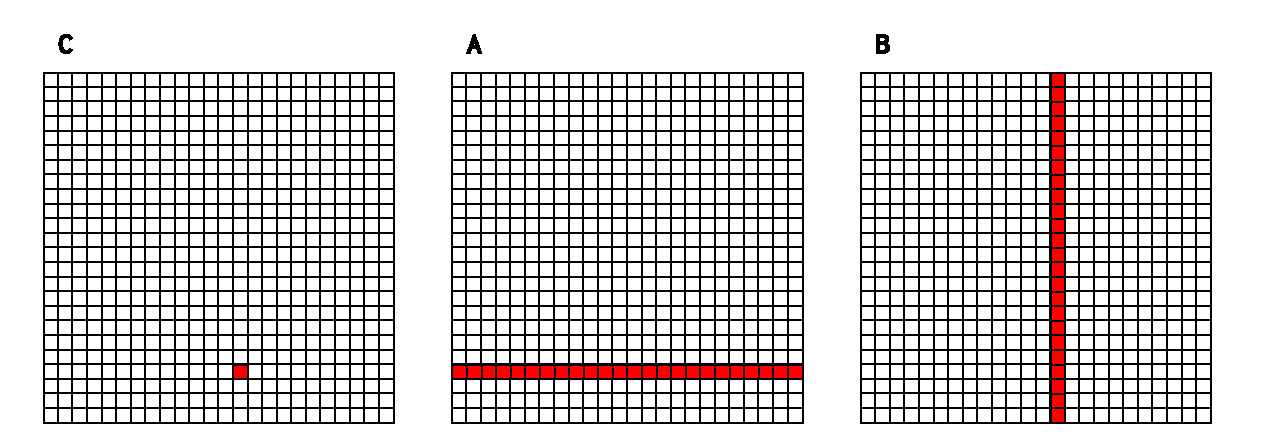
\includegraphics[width=0.75\textwidth]{figures/05-analysis/mm_naive.pdf}
	\captionof{figure}{Visual representation of the multiplication using the naive approach}
	\label{fig:mm_naive}
\end{center}

The naive approach involves three nested loops, iterating over the rows and columns of the matrices:

\begin{center}
\centering
\begin{minipage}{\linewidth}
\begin{lstlisting}[
	style=lstC,
    caption={Naive matrix multiplication implemented in C programming language}
    ]
for (i = 0; i < SIZE; i++) {
	for (j = 0; j < SIZE; j++) {
		for (k = 0; k < SIZE; k++) {
			c[i * SIZE + j] += a[i * SIZE + k] * b[k * SIZE + j];
		}
	}
}
\end{lstlisting}
\end{minipage}
\end{center}

\noindent If the matrices are represented as 1D arrays in memory, the naive approach to matrix multiplication results in poor cache performance due to suboptimal data locality.
The naive algorithm frequently jumps between distant memory locations, leading to cache misses.

\subsubsection*{Block based approach} \label{sec:mmblock}
The block-based approach improves cache performance by dividing the matrices into smaller sub-matrices (blocks) that fit into cache.

\begin{center}
	\centering
	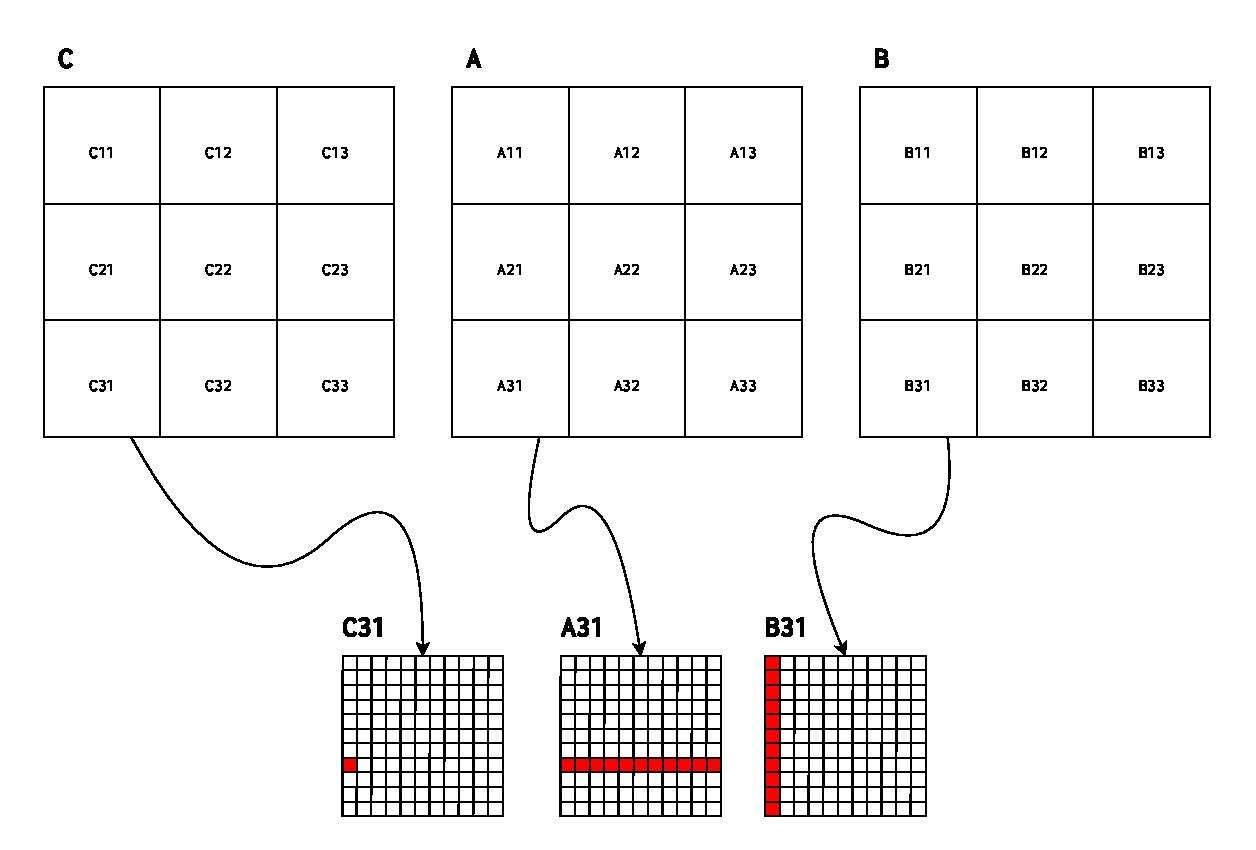
\includegraphics[width=0.75\textwidth]{figures/05-analysis/mm_block.pdf}
	\captionof{figure}{Visual representation of the multiplication using the block based approach}
	\label{fig:mm_block}
\end{center}

\noindent By dividing the large matrix into smaller matrices, data locality is significantly improved, reducing the number of cache misses. This method is particularly effective for
large matrices, where the naive approach would otherwise result in frequent cache evictions. The larger blocks (A11, A12, B11, B12, etc.) are then multiplied and added together.
Selecting the optimal block size is a trade-off. The block size should be small enough to allow the data to fit into the cache but as large as possible to minimize runtime
overhead. Decreasing the block size results in increased runtime overhead because more instructions need to be executed.

\noindent The block-based algorithm has been implemented as follows:
\begin{center}
\centering
\begin{minipage}{\linewidth}
\begin{lstlisting}[
	style=lstC,
    caption={Block based matrix multiplication in C programming language}
    ]
const int B = BLOCK_SIZE;
for (i = 0; i < SIZE; i += B) {
	for (j = 0; j < SIZE; j += B) {
		for (k = 0; k < SIZE; k += B) {
			/* B x B mini matrix multiplications */
			for (i1 = i; i1 < i + B && i1 < SIZE; i1++) {
				for (j1 = j; j1 < j + B && j1 < SIZE; j1++) {
					for (k1 = k; k1 < k + B && k1 < SIZE; k1++) {
						c[i1 * SIZE + j1] += a[i1 * SIZE + k1] * b[k1 * SIZE + j1];
					}
				}
			}
		}
	}
}
\end{lstlisting}
\end{minipage}
\end{center}

\subsection{Linux kernel}
% TODO: this section is a biiit short
The Linux kernel is a core component of many devices, ranging from relatively small microcontrollers to desktop computers and even HPC clusters.
It has been selected as a payload due to its relatively lengthy and memory-access-intensive boot process, such as during the unpacking of initramfs. This process is
characterized by a mix of sequential and random memory access patterns, providing a good benchmark for testing various cache configurations.

\noindent This payload will be used for testing \textit{different hardware configurations}, while the \textit{software remains unchanged}.

\section{Cache model verification}

To validate the model, it was tested against two independent data sources. The first validation was performed using the QEMU TCG Cache Modeling plugin as reference, and the
second test was conducted by using a physical device with built in hardware performance counters. The data input for the cache model implemented in this work was generated using
the Renode framework. This constrains the hardware choice to platforms that are compatible with both QEMU and Renode and are readily available for purchase on the market.

The RISC-V-based SiFive HiFive1 Rev B (\texttt{fu310} SoC with one \texttt{e31} RV32IMAC core) platform has been selected. This platform meets the necessary requirements for
compatibility with both QEMU and Renode, provides extensive documentation including cache parameters, and features built-in hardware performance counters.
The cache configuration for the \texttt{e31} core includes a 16 KiB 2-way set-associative instruction cache with a 32-byte block line size with \textit{random} eviction policy and
no data cache \cite{fe310docs}.
% PZIE this paragraph does not fully work in the context of Linux you mention above

\subsection{Generating cache statistics} \label{sec:gencachestats}

The payload against which the verification was performed is the Zephyr RTOS-based matrix multiplication algorithm (naive approach). Due to the
platform's limited RAM size, the benchmark sample had to be limited to a matrix of size 16 by 16\footnote{Matrices of size $32^2$ resulted in a stack crash (manifesting itself in
a \textit{Load access fault} exception), while sizes $64^2$ and above resulted in a linker failure due to overflowing memory regions.}. The cache usage statistics are gathered
starting from the platform reset, and ended at the \texttt{finished()} symbol entry point, a helper function that marks the end of the matrix multiplication algorithm.\label{snip:measurement_window}

\subsubsection{Novel cache model \& Renode ExecutionTracer} % XXX: replace "novel"
% PIE: Yeah
In order to easily gather cache statistics from the novel cache model using the Renode framework as a trace generation backend, an \textbf{"Automated Renode Cache Test Executor"} % XXX: replace "novel"
toolset was prepared. It is a wrapper, written in bash, that configures, and pipelines the execution of both Renode and Cache model: % XXX: toolset? % PZIE: just "tool" maybe?


\begin{center}
\centering
\begin{minipage}{\linewidth}
\begin{lstlisting}[
    language=Bash,
    caption={Automated Renode Cache Test Executor}
    ]
#!/usr/bin/env bash

DIRECTORY=$1
PRESET=$2
TRACE_DIR="$(realpath traces)"
RESULT_DIR="$(realpath results)"
RENODE_LOG="RENODE_LOG"

for ELF_FILE in "$DIRECTORY"/*.elf; do
	if [ -f "$ELF_FILE" ]; then
		ELF_PATH="$(realpath $ELF_FILE)"
		ELF_FNAME=$(basename -- "$ELF_FILE" .elf)
		TRACE_PATH="$TRACE_DIR/$ELF_FNAME.log"
		RESULT_PATH="$RESULT_DIR/$ELF_FNAME.txt"

		echo "[$(date +%H:%M:%S)] Generating traces using Renode for $ELF_FNAME" tee -a "$RENODE_LOG"

		RENODE_ELF="@$ELF_PATH" RENODE_TRACE="@$TRACE_PATH" renode --console --disable-gui 1>>"$RENODE_LOG" cache.resc &&
		renode_cache_mdl.py "$TRACE_PATH" presets "$PRESET" > "$RESULT_PATH"

		echo "[$(date +%H:%M:%S)] finished" | tee -a "$RENODE_LOG"
		echo "" | tee -a "$RENODE_LOG"
	fi
done
\end{lstlisting}
\end{minipage}
\end{center}
% PZIE What's with the last echo?

% \noindent The Renode script (\texttt{.resc}) file is uses the passed environment variables to set up the simulation.
\noindent The Renode script (\texttt{.resc}) file is designed to set up the simulation environment using the passed environment variables. It loads the platform description from
the \texttt{cache\_platform.repl} file - in this case this file had contained the \texttt{fu310} SoC platform description - and an ELF file specified by the environment variables.


\begin{center}
\centering
\begin{minipage}{\linewidth}
\begin{lstlisting}[
    caption={Renode script for Automated Renode Cache Test Executor}
    ]
set cacheSimulationExecutionCtrl
"""
from Antmicro.Renode.Peripherals.CPU import ICPU
sysbus = self.Machine.SystemBus
cpu = self.Machine.GetPeripheralsOfType(ICPU)[0]

def end_hook(cpu, addr):
    cpu.Pause()
    monitor.Parse("q")

for addr in sysbus.GetAllSymbolAddresses("finished"):
    cpu.AddHook(addr, end_hook)
"""

using sysbus
mach create
machine LoadPlatformDescription @cache_platform.repl
sysbus LoadELF `get_environ RENODE_ELF`

cpu MaximumBlockSize 1
cpu CreateExecutionTracing "tracer" `get_environ RENODE_TRACE` PCAndOpcode
tracer TrackMemoryAccesses

python $cacheSimulationExecutionCtrl
start
\end{lstlisting}
\end{minipage}
\end{center}

\noindent The script was executed with two arguments passed. The first argument sets the directory containing the payload ELF file (or files), and the second argument set the cache preset to \texttt{fu310.e31}:
\begin{verbatim}
./automated_renode_cache_exec.sh elfs/ "fu310.e31"
\end{verbatim}

\noindent The Renode script was executed, and the resulting cache simulation data were saved to a file. These results are presented in Table \ref{table:cache_results}.
% PZIE Why past tense all of a sudden?


\subsubsection{QEMU TCG Cache Modeling plugin}
The QEMU was invoked with the following parameters:
\begin{verbatim}
qemu-system-riscv32 -nographic           \
	-machine sifive_e                       \ # simulate fu310 SoC
	-icount align=off,sleep=off             \ # decouple virtual and host time
	-kernel payload.elf                     \ # payload executable
	-plugin ./contrib/plugins/libcache.so,  \ # use TCG Cache modelling plugin
	        icachesize=16384,               \ # 16 KiB cache size
	        iassoc=2,                       \ # 2-way set-associativity
	        iblksize=32,                    \ # 32 bytes block size
	        evict=rand                      \ # random eviction policy
	-s -S                                     # enable GDB stub and wait for connection
\end{verbatim}

\noindent The virtual platform was then connected to using \texttt{riscv64-zephyr-elf-gdb}, a breakpoint was placed on the \texttt{finished()} symbol, and the execution was started:
\begin{verbatim}
riscv64-zephyr-elf-gdb payload.elf   \
	-ex 'target extended-remote :1234'  \ # connect to QEMU GDB stub
	-ex 'break finished'                \ # stop execution upon entering finished()
	-ex 'continue'                        # start executing the payload
\end{verbatim}

\noindent After the program halted at the breakpoint, the QEMU simulator was terminated, and the resulting cache simulation data were saved to a file. These results are presented in % TODO: too much passive voice? this reads weeeird
Table \ref{table:cache_results}.


\subsubsection{Hardware Performance Counters}
The \texttt{fu310} system-on-chip has a built-in Hardware Performance Monitor (HPM), that can be configured to measure a variety of performance statistics. These counters are configured
using the RISC-V Control and Status Registers (CSRs) \cite{fe310docs, riscvisa}.
Although the Zephyr RTOS provides a set of C macros to interface with CSRs, it is not possible to use this interface to inject the HPM configuration at the early stages of the
operating system bringup - a necessary step to collect the cache statistics for the measurement window described in Section (\ref{snip:measurement_window}). To work around this limitation,
a \textit{simplified} Zephyr RTOS bootup sequence for the RISC-V platform is examined:

\begin{verbatim}
arch/riscv/core/reset.S
__reset -> __initialize -> boot_first_core -> z_prep_c (first C code)

arch/riscv/core/prep_c.c
z_prep_c() -> z_bss_zero() -> z_data_copy() -> z_cstart() (zephyr kernel)
\end{verbatim}

\noindent The \texttt{z\_prep\_c} function was chosen as a suitable place to insert the HPM configuration code because initializing it earlier in \texttt{reset.S} (written in
assembly) offers no significant advantage, and,  writing the configuration in C provides better readability, maintainability, and ease of configuration. The performance counter
was set up and cleared according to the RISC-V Instruction Set Manual - Privileged Architecture:

\begin{center}
\centering
\begin{minipage}{\linewidth}
\begin{lstlisting}[
	style=lstC,
    caption={RISC-V Hardware Performance Monitor configuration}
    ]
void z_prep_c(void)
{
#ifdef HPM_INIT
  unsigned int val = 0u;
  unsigned int bitmask = (1UL << 8) | (2UL); /* EVENTID:8 EVENTCLASS:2 */
  __asm__ volatile("csrr %0, mhpmevent4" : "=r"(val));
  val = (val & ~bitmask) | bitmask;
  __asm__ volatile("csrw mhpmevent4, %0" : : "r"(val));
  __asm__ volatile("csrw mhpmcounter4, zero");
  __asm__ volatile("csrw mhpmcounter4h, zero");
#endif
  z_bss_zero();
  z_data_copy();
  z_cstart();
  CODE_UNREACHABLE;
}
\end{lstlisting}
\end{minipage}
\end{center}

\noindent To comply with the measurement window described in Section (\ref{snip:measurement_window}), the performance counters are later accessed, and their values are read in the
\textit{finished()} function:

\begin{center}
\centering
\begin{minipage}{\linewidth}
\begin{lstlisting}[
	style=lstC,
    caption={Accessing RISC-V HPM counters}
    ]
void __attribute__ ((noinline)) finished(void)
{
#ifdef HPM_INIT
	unsigned long lo = 0l;
	__asm__ volatile("csrr %0, mhpmcounter4" : "=r"(lo));
	printf("hpm4 data: %lu\n", lo);
#else
	__asm__ volatile("addi x0, x0, 0");
#endif
}
\end{lstlisting}
\end{minipage}
\end{center}

\noindent The sample was then compiled and flashed onto the hardware target using the \texttt{west} utility. The performance counter results are presented in Table \ref{table:cache_results}.

\subsection{Verification results}

\begin{center}
\begin{table}[h!]
\centering
\begin{tabular}{|l|c|c|c|c|}
\hline
\textbf{Environment} & \textbf{Accesses} & \textbf{Misses} & \textbf{Hits} & \textbf{HMR} \\ \hline
Cache model + Renode generated trace    & 91468        & 291         & 91177 & 99.68\%    \\ \hline
QEMU TCG Cache Modeling Plugin          & 91470        & 292         & 91178 & 99.68\%    \\ \hline
Hardware performance counters           & -            & 217         & - & -			  \\ \hline % TODO: i think it might be possible to get the accesses using the minstret csr?
\end{tabular}
\caption{Instruction accesses and misses generated by the Cache Model + Renode Traces, QEMU TCG Cache modelling plugin and HPMs.}
\label{table:cache_results}
\end{table}
\end{center}

\noindent The verification results show a high degree of similarity between the Cache model using Renode-generated traces and the QEMU TCG Cache Modeling Plugin, with both environments
reporting nearly identical instruction accesses, misses, and hit to miss ratios. The discrepancy in the number of cache misses observed in the hardware performance counters,
compared to the emulated cache models, could be attributed to the later initialization of the hardware performance counters. As a result, some initial instructions might not have
been counted. It is important to note that it is impossible to obtain the instruction access count from the HPMs, as there is no specific counter for this purpose.

\section{Benchmarks}

The benchmarks were performed using the simulated HiFive Unmatched platform (\texttt{fu740} SoC with one \texttt{s7} RV64IMAC and four \texttt{u74} RV64GC cores) \cite{fu740docs}.
This platform was chosen due to its support for both the Zephyr and Linux operating systems, and its relatively large RAM size, which allows for the execution of more substantial
and cache-intensive payloads. Additionally, this machine platform description is provided with the Renode framework.
The matrix multiplication payloads will be used to analyze the impacts of optimizing payload configuration on cache usage, while the Linux boot process will be used to measure the
impact of changing cache configurations.

\subsection{Matrix multiplication}

The benchmarks for matrix multiplication use the same code and measurement window as the described in Section (\ref{sec:gencachestats}) - measurement begins as soon
as the platform is initialized, and ends upon reaching the \texttt{finished()} symbol.
The following payload configurations were tested:
\begin{itemize}
	\item Naive approach with matrix sizes of $8^2$, $16^2$, $32^2$, $64^2$, $128^2$, and $256^2$.
	\item Block-based approach with matrix sizes of $16^2$, $32^2$, $64^2$, $128^2$, and $256^2$. For each matrix size, block sizes were chosen such that $bs = 2^n$ where
		$n \in \{3, 4, \ldots, \log_2(\text{size}) - 1\}$. For example, for a matrix size of $256^2$, block sizes of $8$, $16$, $32$, $64$, and $128$ were used.
\end{itemize}

\noindent The benchmarks will focus solely on the first level of data cache (abbreviated to \texttt{L1D\$}), as changes in algorithm and matrix size have not produced any
significant differences in the instruction cache results. Additionally, the \textit{Instruction Executed} statistic is provided to analyze the impact of block size on the number of
executed instructions by the CPU.

\subsubsection{Naive approach}

\begin{center}
\begin{table}[h!]
\centering
\begin{tabular}{|c|c|c|c|c|c|}
\hline
\textbf{Size} & \textbf{Instr. Exec.} & \textbf{Mem. Acc.} & \textbf{L1D\$ Misses} & \textbf{L1D\$ Hits} & \textbf{L1D\$ HMR} \\ \hline
8 & 42594 & 12451 & 176 & 12275 & 98.59\% \\ \hline
16 & 98458 & 32163 & 224 & 31939 & 99.30\% \\ \hline
32 & 465156 & 168355 & 415 & 167940 & 99.75\% \\ \hline
64 & 3078628 & 1171875 & 2928 & 1168947 & 99.75\% \\ \hline
128 & 22707108 & 8855971 & 1768972 & 7086999 & 80.03\% \\ \hline
256 & 174620452 & 68952483 & 17320212 & 51632271 & 74.88\% \\ \hline
\end{tabular}
\caption{Performance metrics for matrix multiplication - naive approach}
\label{tab:performance_metrics}
\end{table}
\end{center}

\subsubsection{Block based approach}

\begin{center}
\begin{table}[!htbp]
\centering
\begin{tabular}{|c|c|c|c|c|c|}
\hline
\textbf{Block Size} & \textbf{Instr. Exec.} & \textbf{Mem. Acc.} & \textbf{L1D\$ Misses} & \textbf{L1D\$ Hits} & \textbf{L1D\$ HMR} \\ \hline
8 & 124411 & 32323 & 223 & 32100 & 99.31\% \\ \hline
\end{tabular}
\caption{Performance metrics for matrix multiplication - block based approach - matrix size 16}
\label{tab:performance_metrics_16}
\end{table}
\end{center}

\begin{center}
\begin{table}[!htbp]
\centering
\begin{tabular}{|c|c|c|c|c|c|}
\hline
\textbf{Block Size} & \textbf{Instr. Exec.} & \textbf{Mem. Acc.} & \textbf{L1D\$ Misses} & \textbf{L1D\$ Hits} & \textbf{L1D\$ HMR} \\ \hline
8 & 681401 & 168517 & 410 & 168107 & 99.76\% \\ \hline
16 & 665005 & 168532 & 414 & 168118 & 99.75\% \\ \hline
\end{tabular}
\caption{Performance metrics for matrix multiplication - block based approach - matrix size 32}
\label{tab:performance_metrics_32}
\end{table}
\end{center}

\begin{center}
\begin{table}[!htbp]
\centering
\begin{tabular}{|c|c|c|c|c|c|}
\hline
\textbf{Block Size} & \textbf{Instr. Exec.} & \textbf{Mem. Acc.} & \textbf{L1D\$ Misses} & \textbf{L1D\$ Hits} & \textbf{L1D\$ HMR} \\ \hline
8 & 4838437 & 1172037 & 3015 & 1169022 & 99.74\% \\ \hline
16 & 4722673 & 1172054 & 2849 & 1169205 & 99.76\% \\ \hline
32 & 4661425 & 1172054 & 3084 & 1168970 & 99.74\% \\ \hline
\end{tabular}
\caption{Performance metrics for matrix multiplication - block based approach - matrix size 64}
\label{tab:performance_metrics_64}
\end{table}
\end{center}

\begin{center}
\begin{table}[!htbp]
\centering
\begin{tabular}{|c|c|c|c|c|c|}
\hline
\textbf{Block Size} & \textbf{Instr. Exec.} & \textbf{Mem. Acc.} & \textbf{L1D\$ Misses} & \textbf{L1D\$ Hits} & \textbf{L1D\$ HMR} \\ \hline
8 & 36913565 & 8856133 & 61860 & 8794273 & 99.3\% \\ \hline
16 & 35988573 & 8856150 & 33847 & 8822303 & 99.62\% \\ \hline
32 & 35562485 & 8856152 & 25949 & 8830203 & 99.71\% \\ \hline
64 & 35325616 & 8856150 & 140394 & 8715756 & 98.41\% \\ \hline
\end{tabular}
\caption{Performance metrics for matrix multiplication - block based approach - matrix size 128}
\label{tab:performance_metrics_128}
\end{table}
\end{center}

\begin{center}
\begin{table}[!htbp]
\centering
\begin{tabular}{|c|c|c|c|c|c|}
\hline
\textbf{Block Size} & \textbf{Instr. Exec.} & \textbf{Mem. Acc.} & \textbf{L1D\$ Misses} & \textbf{L1D\$ Hits} & \textbf{L1D\$ HMR} \\ \hline
8 & 288790285 & 68952645 & 451736 & 68500909 & 99.34\% \\ \hline
16 & 281395673 & 68952664 & 253546 & 68699118 & 99.63\% \\ \hline
32 & 277988449 & 68952664 & 1617083 & 67335581 & 97.65\% \\ \hline
64 & 276351989 & 68952664 & 14314624 & 54638040 & 79.24\% \\ \hline
128 & 275419880 & 68952679 & 17078642 & 51874037 & 75.23\% \\ \hline
\end{tabular}
\caption{Performance metrics for matrix multiplication - block based approach - matrix size 256}
\label{tab:performance_metrics_256}
\end{table}
\end{center}

\subsection{Linux kernel boot sequence}

The benchmarks will focus on both the first level of data cache (abbreviated as \texttt{L1D\$}) and the first level instruction cache (abbreviated as \texttt{L1I\$}). The software
configuration will remain unchanged, with the only variable being the simulated cache configuration. The trace gathering window will commence as soon as the Linux kernel takes
control of the CPU and will conclude upon reaching the user-space login prompt. The following configurations have been tested:

\begin{itemize}
    \item Standard platform configuration: 32 KiB instruction and data caches, 64-byte cache blocks, 4-way set associative instruction cache, and 8-way set associative data cache.
    \item Modified cache sizes: 64 KiB (2x), 128 KiB (4x), 16 KiB (0.5x), 8 KiB (0.25x).
    \item Reduced associativity: 2-way set associative instruction cache, 4-way set associative data cache.
    \item Fully associative caches: Fully associative instruction and data caches.
    \item Modified cache block sizes: 128 bytes (2x), 32 bytes (0.5x).
\end{itemize}

\noindent For every test run, the total number of instructions executed was 33,470,111, with 775,974 memory accesses (reads: 41,937, writes: 35,659).

\begin{center}
\begin{table}[!htbp]
\centering
\begin{tabular}{|c|c|c|c|c|c|}
\hline
\textbf{Cache configuration}  & \textbf{L1I\$ Misses} & \textbf{L1D\$ Misses} & \textbf{L1I\$ HMR} & \textbf{L1D\$ HMR}\\ \hline
Standard configuration & 3648528 & 8238 & 98.91\% & 98.94\% \\ \hline
Doubled caches size & 1363438 & 8237 & 99.59\% & 98.94\% \\ \hline
Quadrupled caches size & 438583 & 8237 & 99.87\% & 98.94\% \\ \hline
Halved caches size & 6844164 & 8237 & 97.96\% & 98.94\% \\ \hline
Quartered caches size & 9970037 & 8239 & 97.02\% & 98.94\% \\ \hline
Doubled caches block size & 3253047 & 4130 & 99.03\% & 99.47\% \\ \hline
Halved caches block size & 4600941 & 16451 & 98.63\% & 97.88\% \\ \hline
Halved associativity & 4424764 & 8241 & 98.68\% & 98.94\% \\ \hline
Fully associative cache & 2896796 & 8237 & 99.13\% & 98.94\% \\ \hline
\end{tabular}
\caption{Performance metrics for various cache configurations - Linux boot}
\label{tab:performance_metrics_linux}
\end{table}
\end{center}

\section{Benchmark conclusions}

\subsection*{Matrix Multiplication}

The table with cache statistics for the naive approach (Table \ref{tab:performance_metrics}) displays the effects of non-cache optimized algorithms. The data reveals a significant
increase in L1D\$ cache misses as matrix size grows, which highlights the inefficiency of the naive method in utilizing cache memory effectively. The hit rate drops markedly from
98.59\% for the smallest matrix to 74.88\% for the largest, demonstrating the strain placed on the cache by larger matrices. This inefficiency leads to a higher number of memory
accesses and executed instructions, resulting in suboptimal performance.

\begin{center}
	\centering
	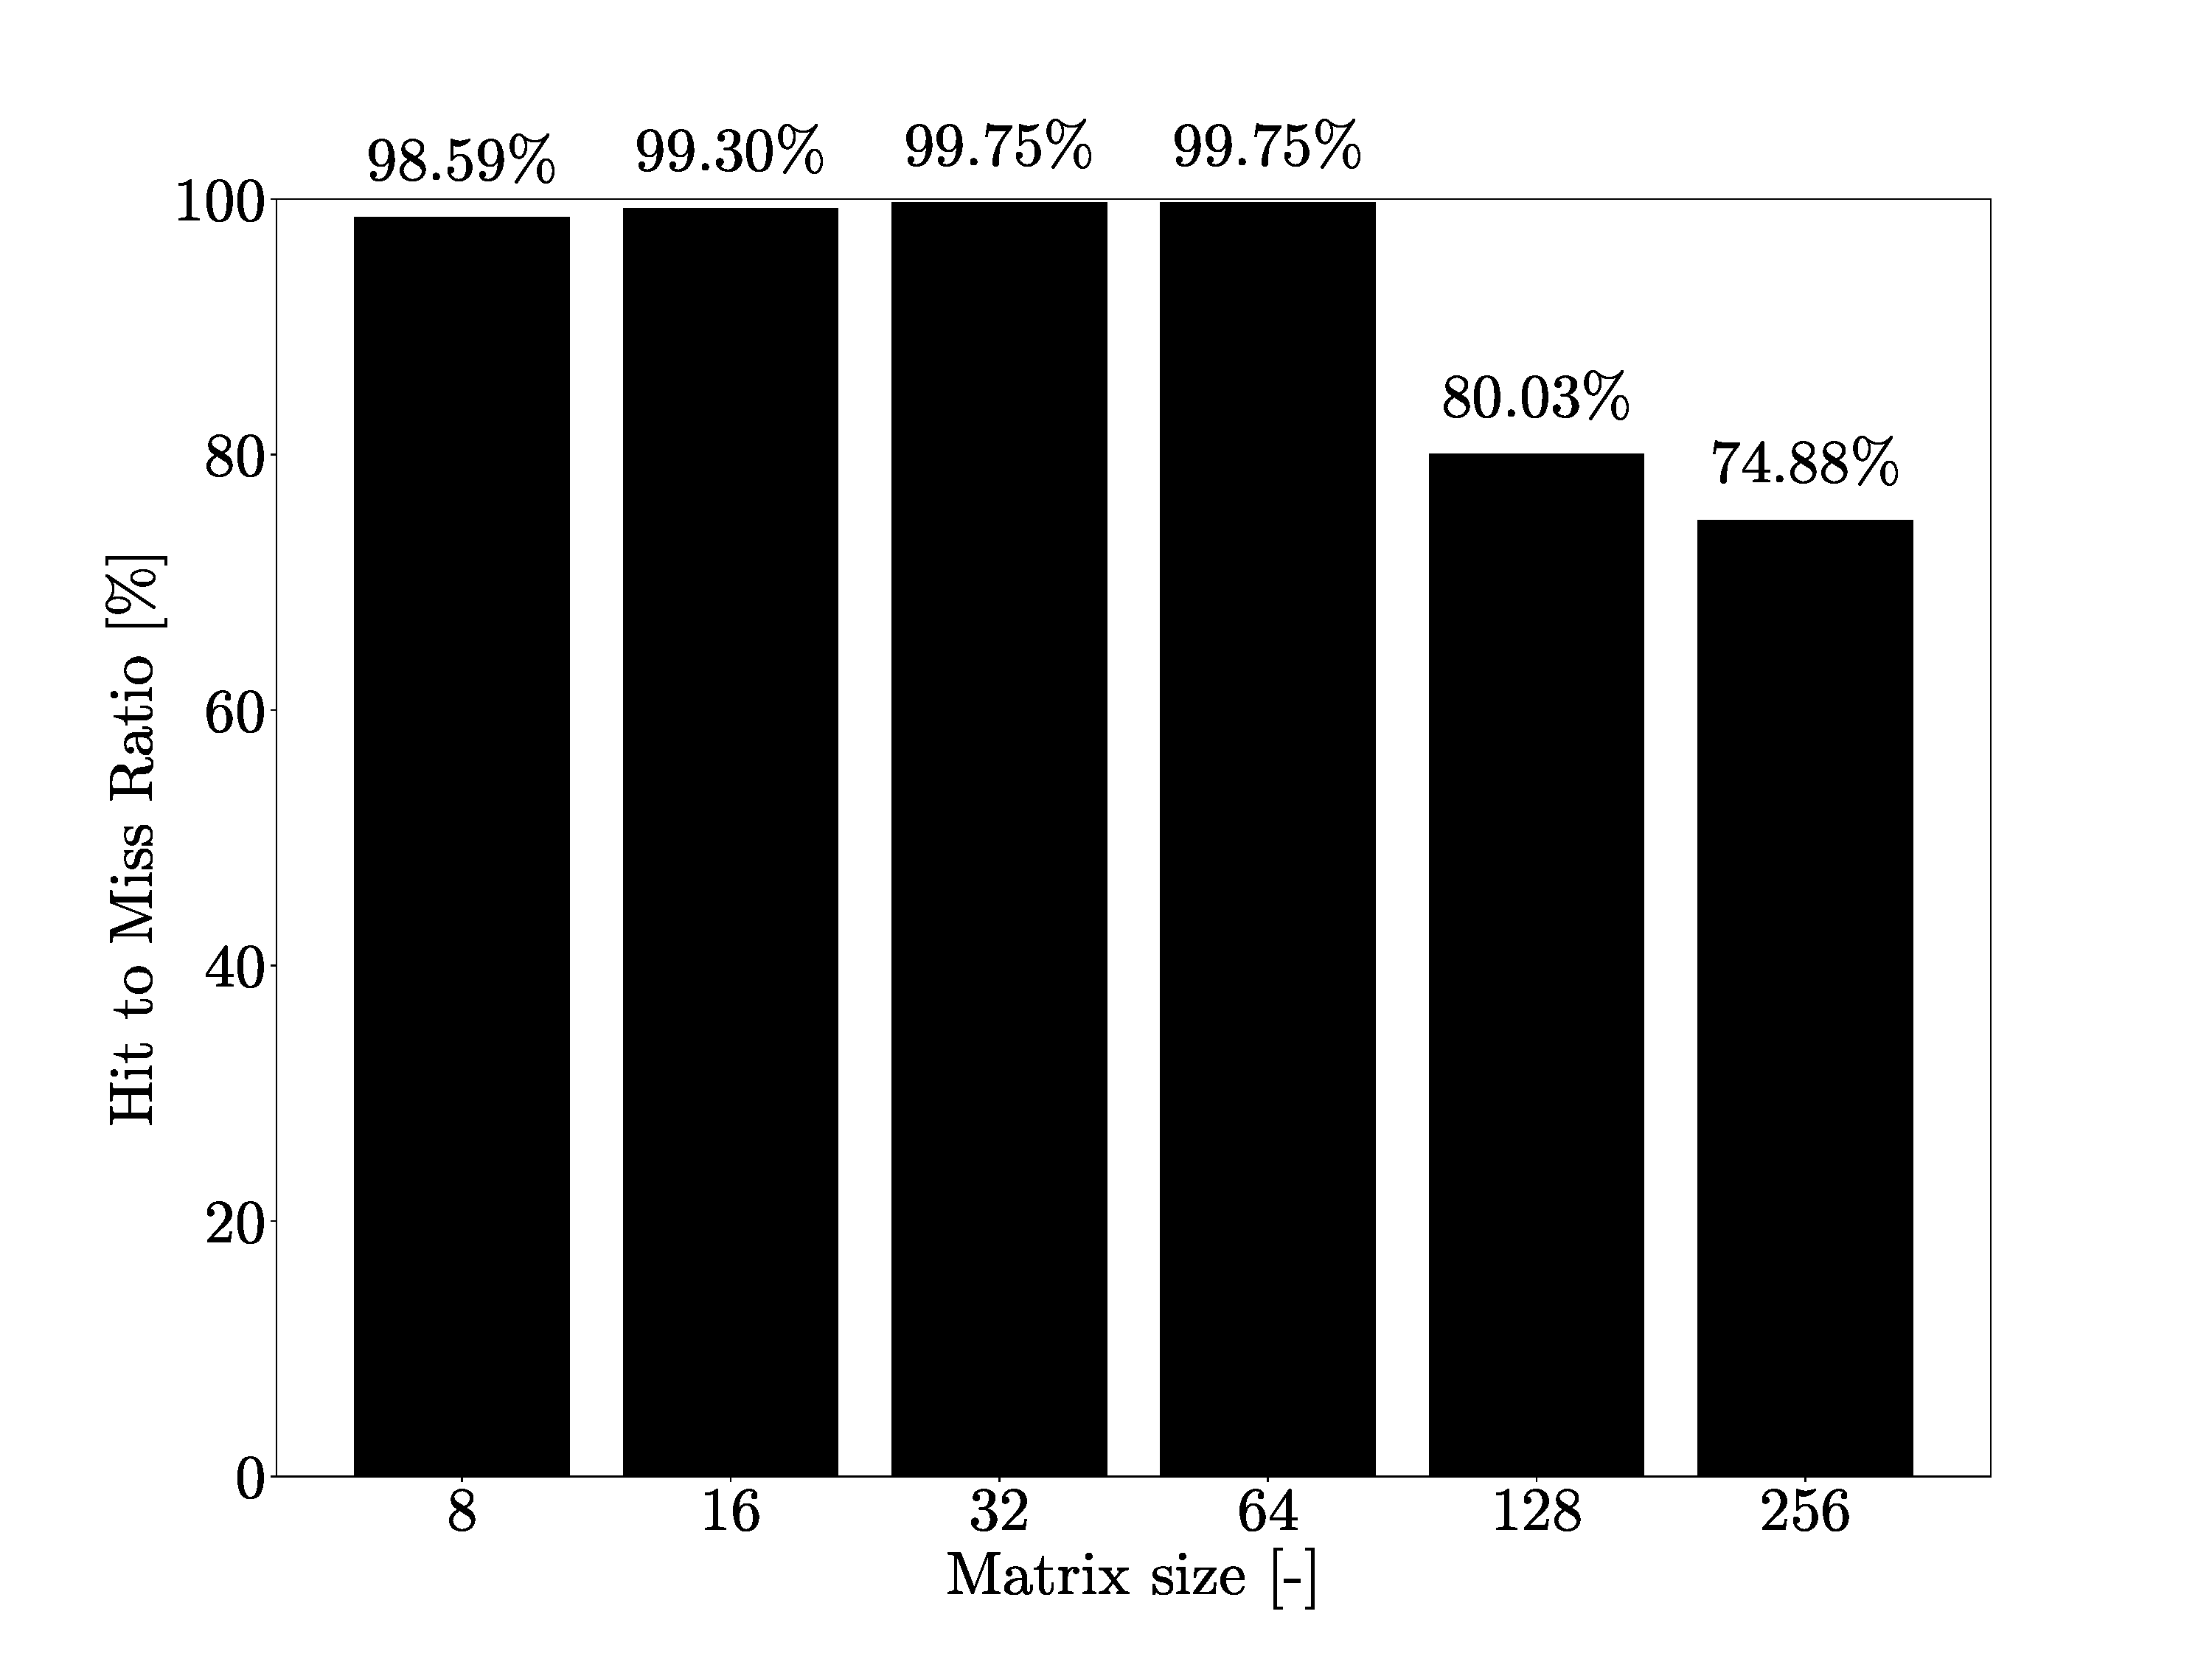
\includegraphics[width=0.75\textwidth]{figures/05-analysis/mm_naive_results.pdf}
	\captionof{figure}{HMR visualization for the naive matrix multiplication algorithm}
	\label{fig:mm_naive_results}
\end{center}

\noindent The cache-optimized block-based approach, detailed in Tables (\ref{tab:performance_metrics_16}) to (\ref{tab:performance_metrics_256}), demonstrates significantly
improved cache utilization. By dividing the matrices into smaller blocks, this method enhances data locality and reduces cache misses, particularly for larger matrices. The block
size plays a critical role in optimizing cache performance, as reflected in the varying hit rates. For instance, with a matrix size of \( 128^2 \), a block size of 32 achieves the
highest hit rate of 99.71\%, substantially better than the naive approach.

\begin{figure}[!htbp]
    \centering
    \begin{subfigure}{0.5\textwidth}
      \centering
      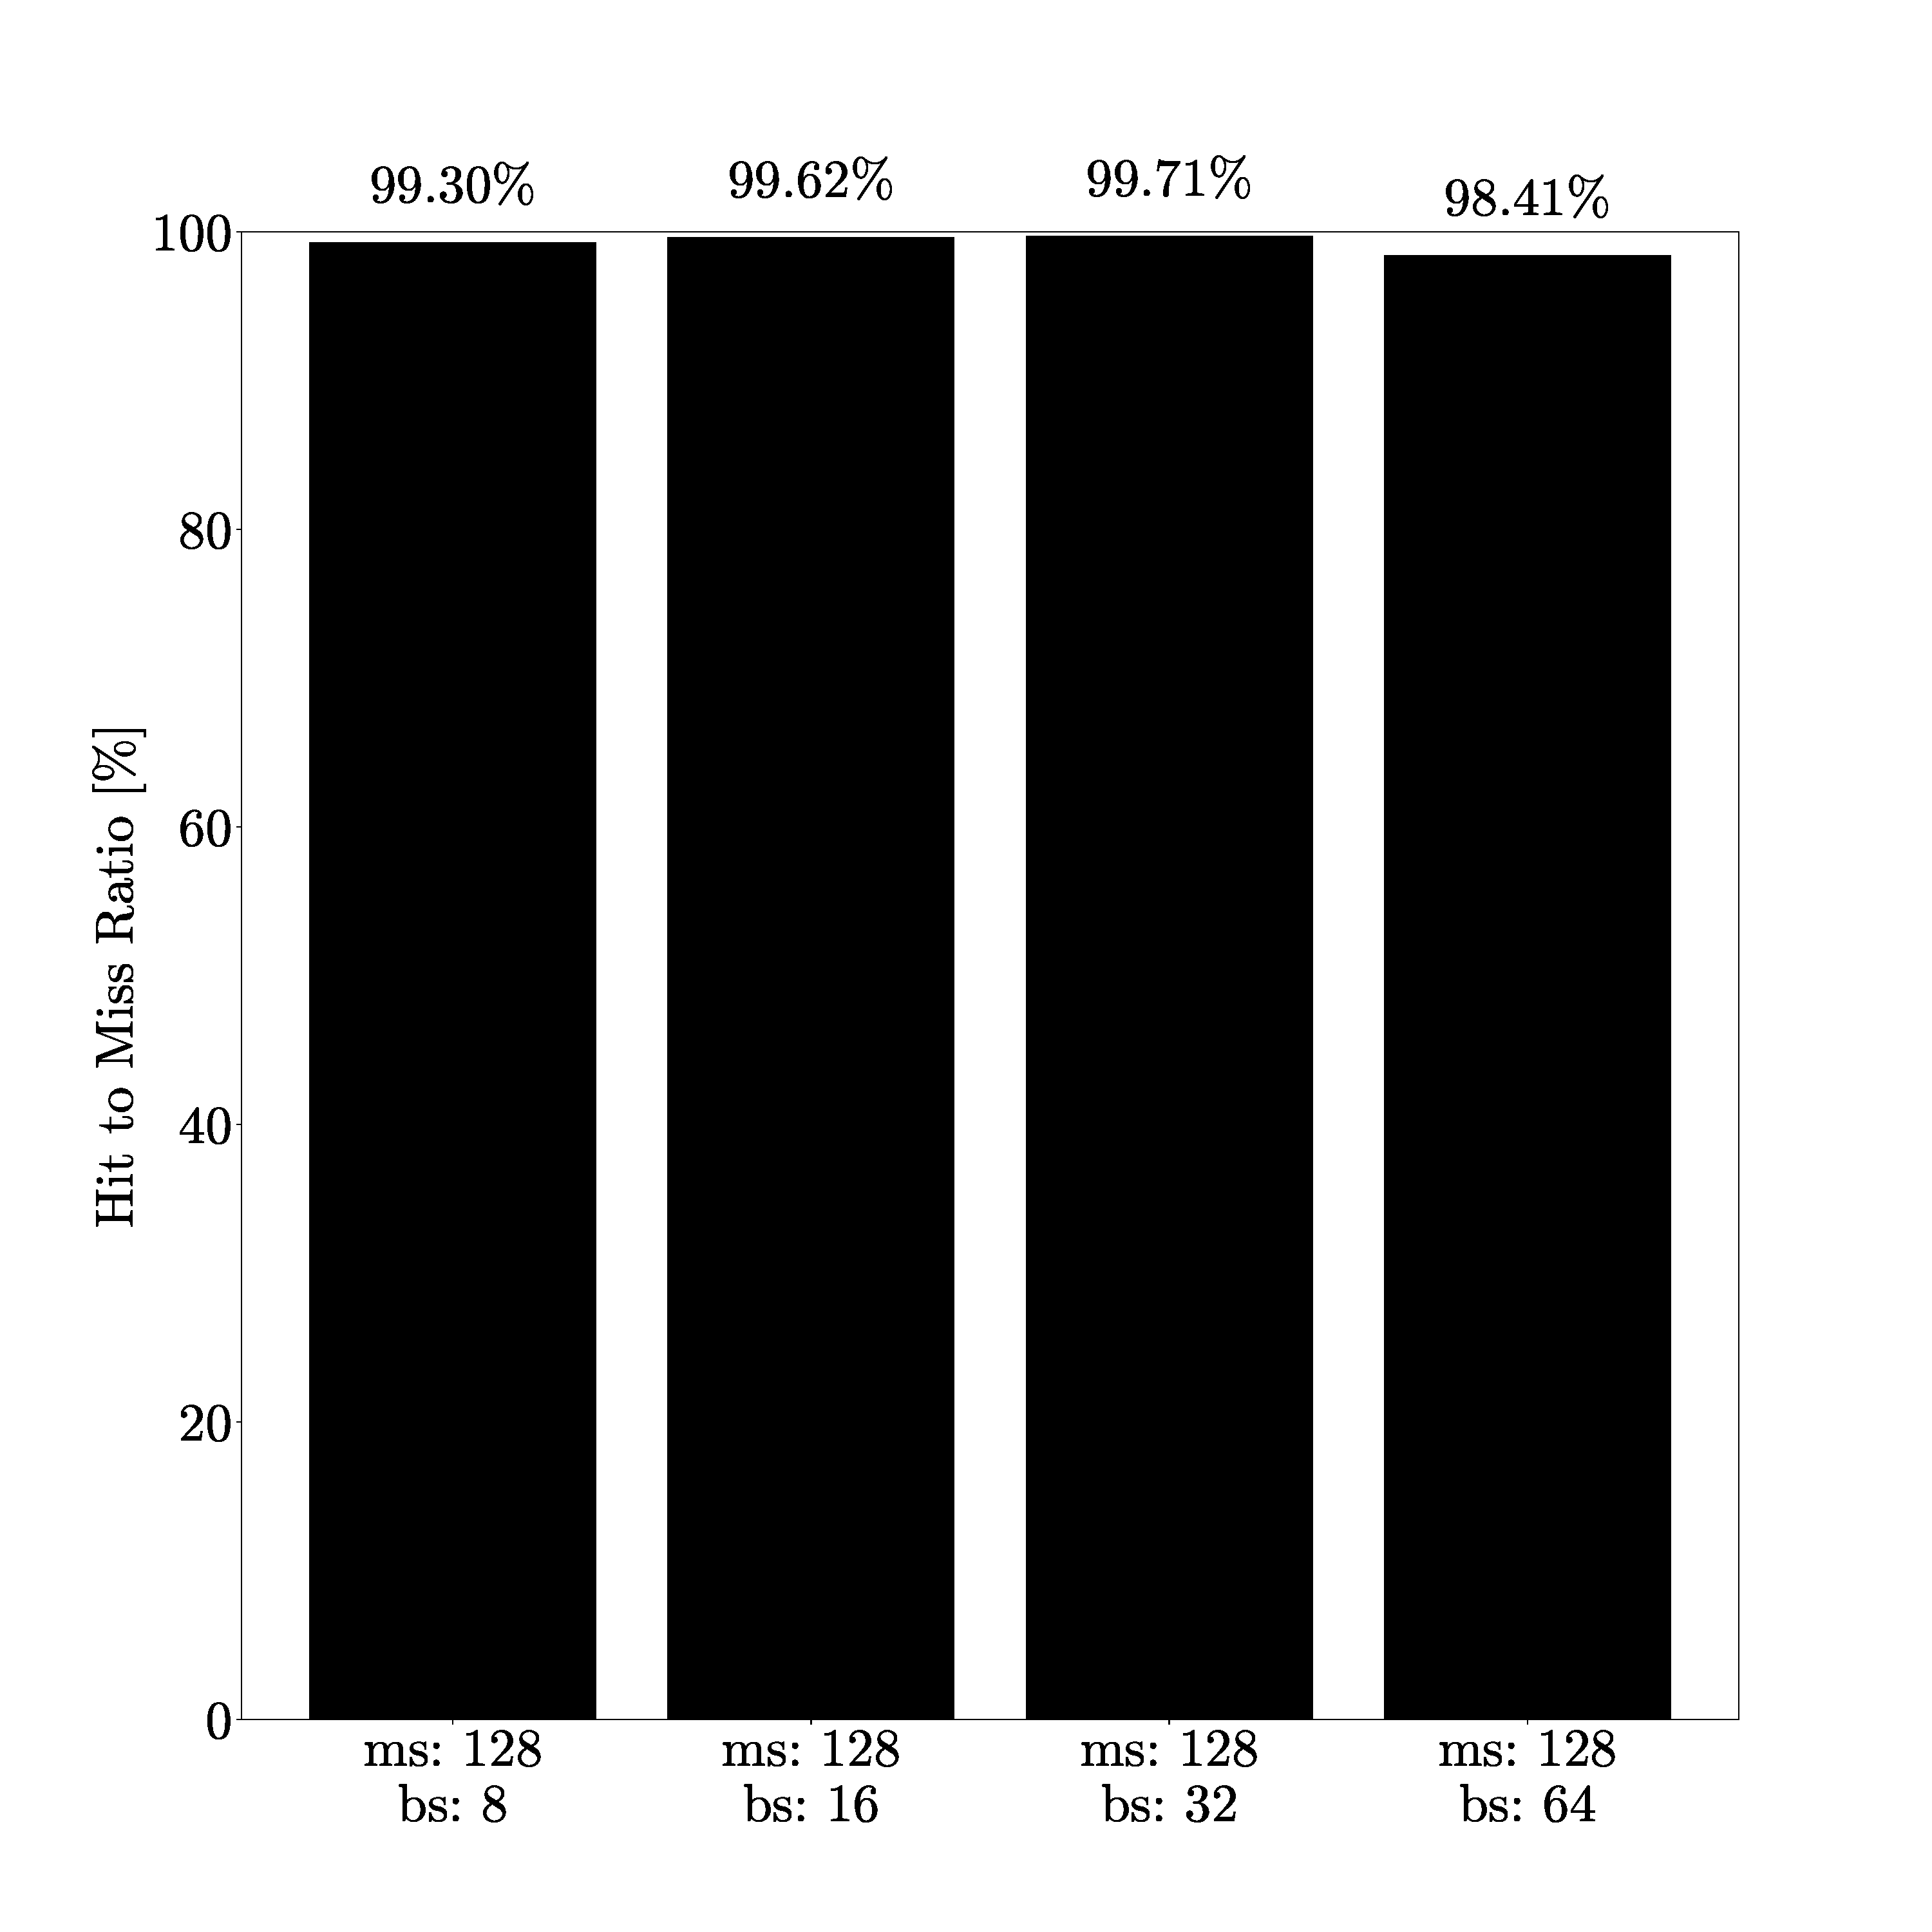
\includegraphics[width=1\linewidth]{figures/05-analysis/block_ms128.pdf}
    \end{subfigure}%
    \begin{subfigure}{0.5\textwidth}
      \centering
      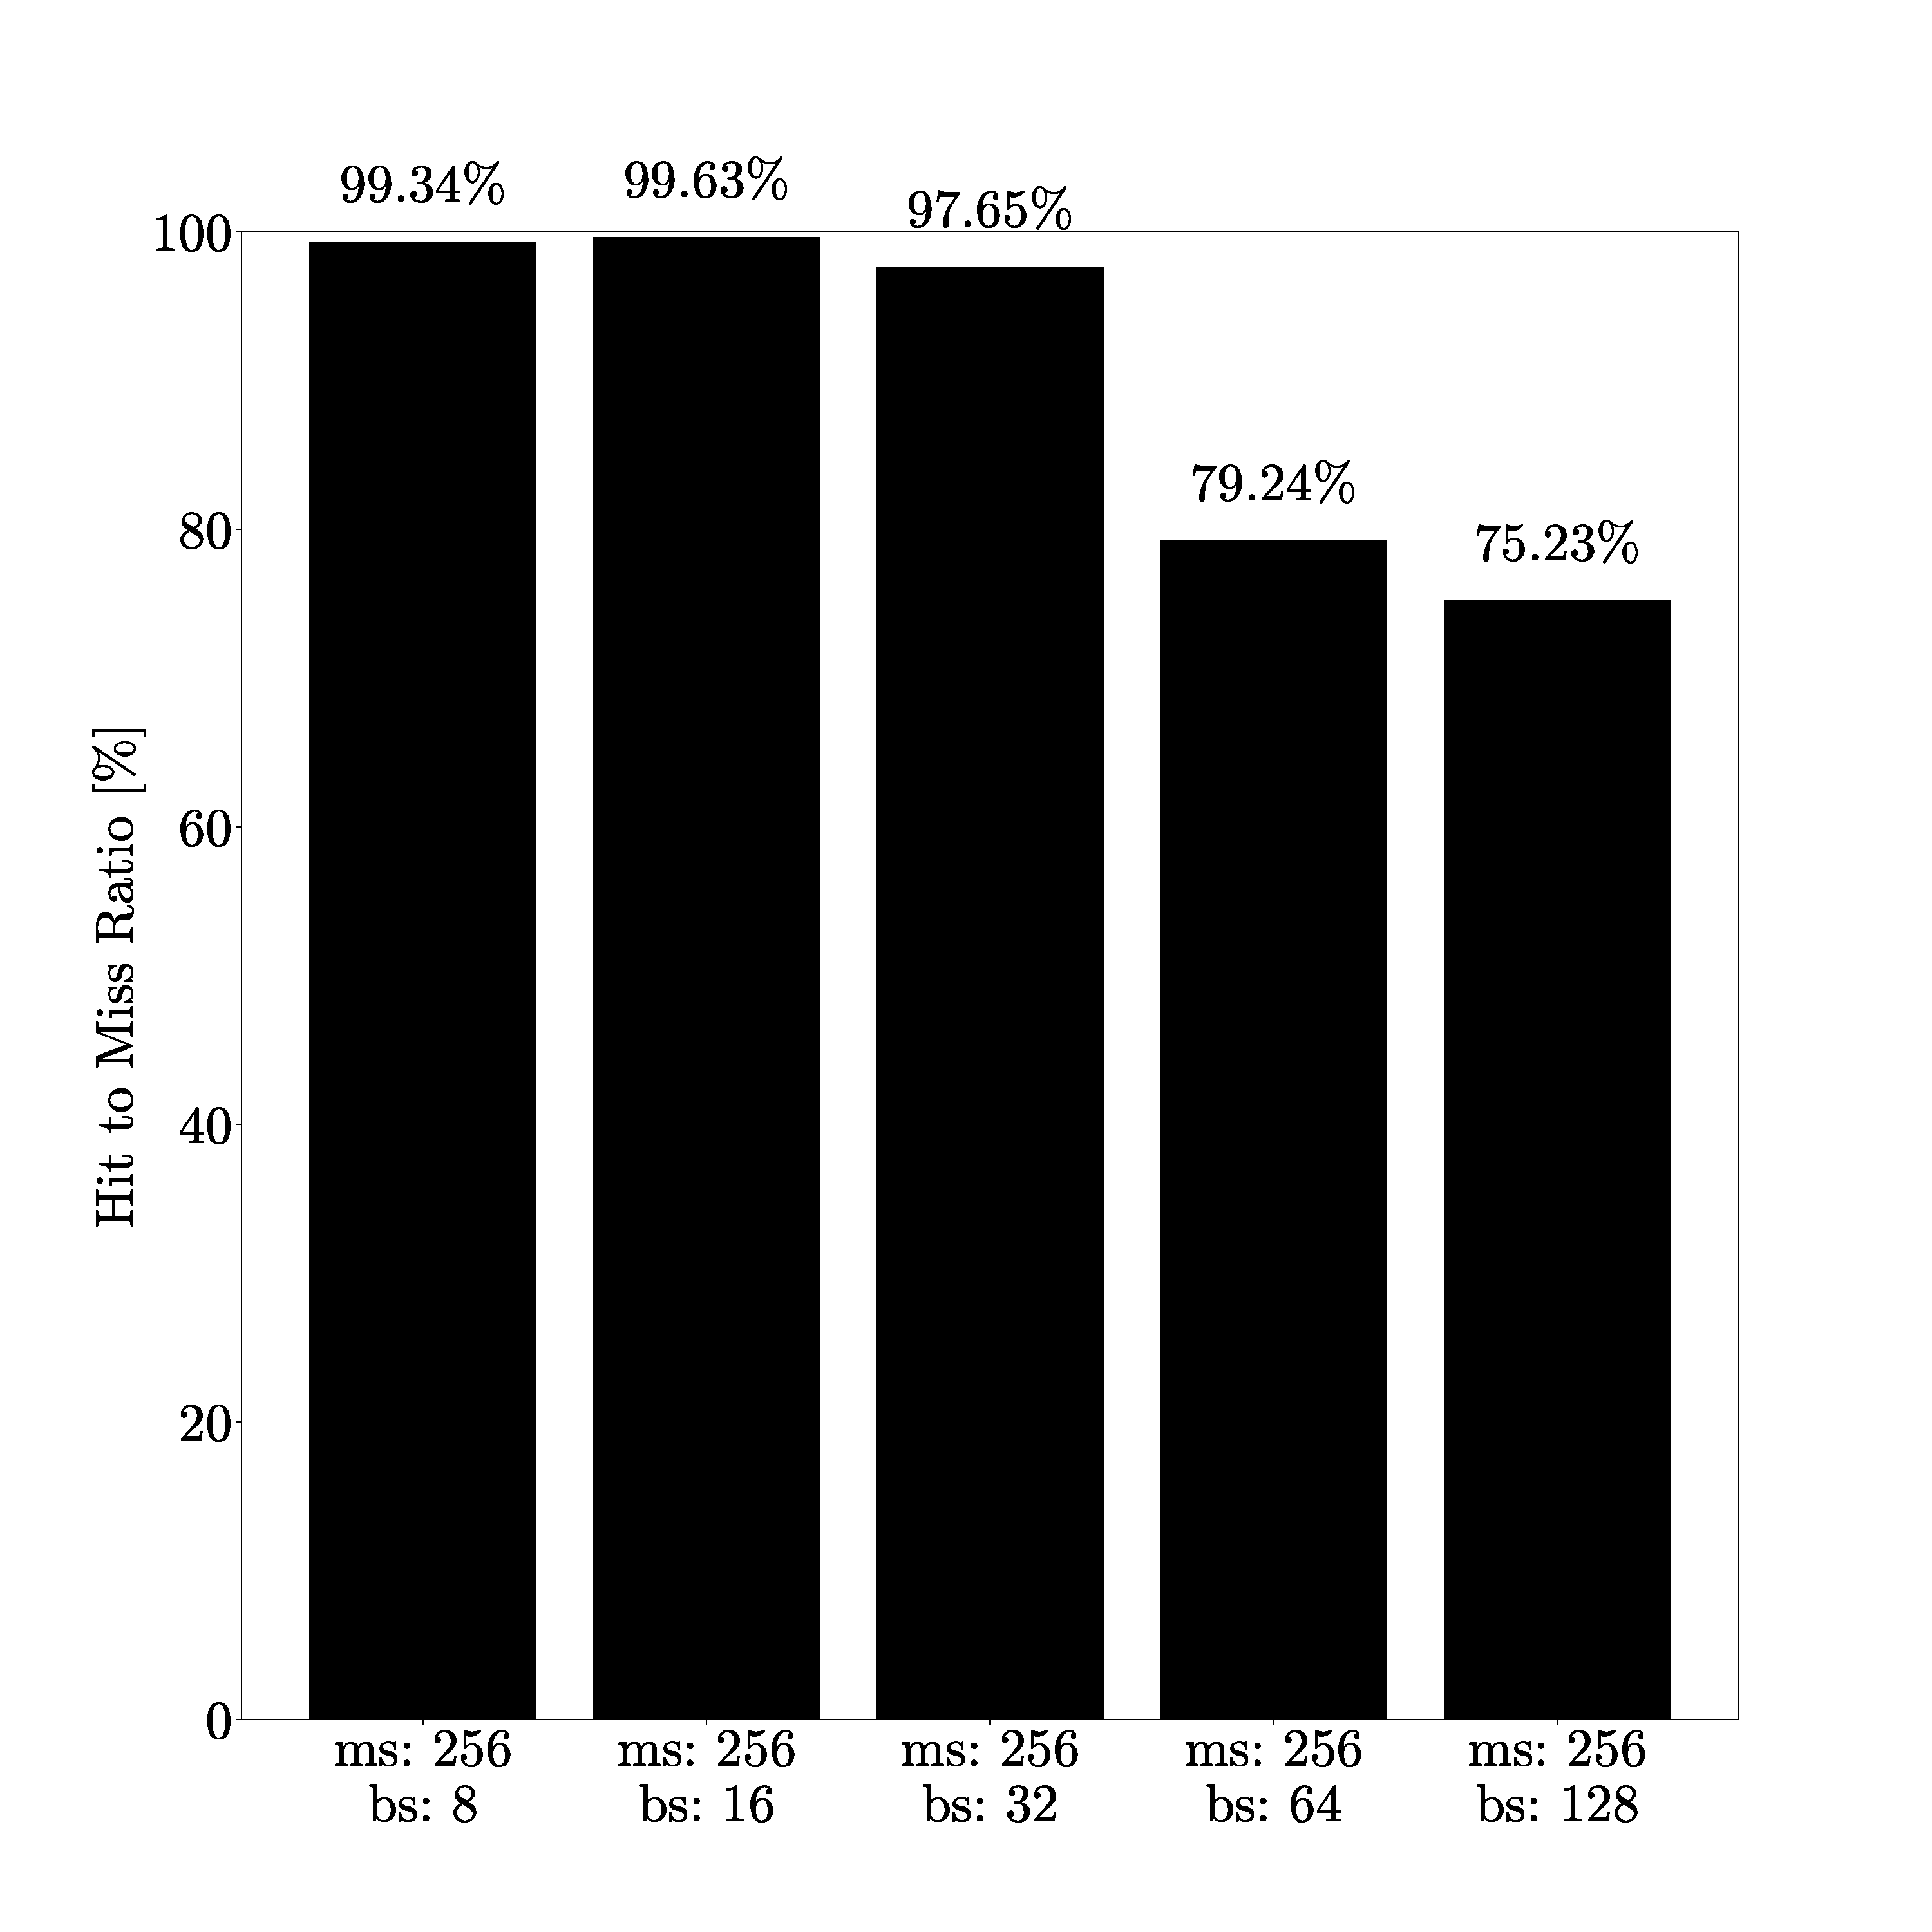
\includegraphics[width=1\linewidth]{figures/05-analysis/block_ms256.pdf}
    \end{subfigure}
    \caption{HMR visualization for a block-based algorithm for matrices of sizes 128 and 256 with various block sizes}
\end{figure}

\noindent It is important to note that decreasing block size has caused an increase in the total instructions executed. For example, the naive approach for matrix size \( 256^2 \) required
174,620,452 instructions, while the block-based approach with block size of 32 required 277,988,449 instructions - a 59\% increase. Overall, the amount of instructions executed
increases as the block size decreases, with block sizes of 8, 32, and 128 requiring 288,790,285 (65.4\% increase), 277,988,449 (59.2\% increase), and 275,419,880 (57.7\% increase)
instructions, respectively.

\subsection*{Linux kernel boot sequence} \label{sec:linux_boot_perf_conc}

Increasing the cache size has reduced the number of cache misses, doubling the instruction cache size decreased misses by approximately 62.6\% (from 3,648,528 to 1,363,438), and
quadrupling it further reduced misses by about 87.9\% (down to 438,583). Decreasing the cache size leads to a significant rise in cache misses, halving the instruction cache size
resulted in an 87.5\% increase in misses (to 6,844,164), and reducing it to a quarter led to an increase of 173.4\% (9,970,037). Modifications of cache size had very little to no
effect on the data cache.

Adjusting the cache block size greatly influenced both caches. Doubling the block size from 64 bytes to 128 bytes has reduced L1D\$ cache misses by approximately 49.9\% (from 8,238
to 4,130) and L1I\$ cache misses by 10.8\% (from 3,648,528 to 3,253,047). Decreasing the block size to 32 bytes resulted in a 99.6\% increase in L1D\$ cache misses (to 16,451) and
L1I\$ cache misses by 26.2\% (to 4,600,941).

Halving the associativity of the instruction cache increased L1I\$ cache misses by 21.6\% (to 4,424,764). Using a fully associative cache reduced L1I\$ cache misses by 20.6\% (to
2,896,796). Changing the mapping configuration had little to no effect on the data cache.


\chapter{Conclusions}

\section{Future work}


%--------------------------------------
% Literatura
%--------------------------------------

\bibliographystyle{unsrt}{\raggedright\sloppy\small\bibliography{bibliografia}}

%--------------------------------------
% Dodatki
%--------------------------------------

\cleardoublepage\appendix%
\newpage
% Removing all includes from this section breaks some conditional
\if

\lstlistoflistings
\clearpage
\listoffigures
\clearpage
\listoftables

\begin{appendices}
   \chapter{Definitions}

\section{Creating and configuring Renode virtual platform configuration files} \label{app:creating_renode_platforms}

The Renode framework uses two types of files to define and configure the simulated virtual platform:

\begin{itemize}
	\item \textbf{Platform description}:
	\item \textbf{Renode scripts}:
\end{itemize}

\end{appendices}

%--------------------------------------
% Informacja o prawach autorskich
%--------------------------------------

\ppcolophon

\end{document}
